\section*{DFS with Timing and Properties}

Recall that the DFS-with-timing algorithm gives an interval $[pre,post]$ for each vertex.
For two vertices $v_i,v_j\in V$, their corresponding intervals can either be
\emph{disjoint}, i.e., the two intervals do not overlap, or \emph{nested}, i.e.,
one interval is within the other. See Figure~\ref{fig:interval}.
But two intervals cannot be \emph{partially overlapping}. Why? This is because
the explore funtion is recursive. There are only two possiblities
that $pre[i] < pre[j]$. The first one is that explore $v_j$ is \emph{within} explore $v_i$;
in this case the recursive behaviour of explore leads to that $post[j] < post[i]$,
as explore $v_j$ must return/terminate first and then explore $v_i$ will return/terminate.
This case corresponds to that the two intervals are nested.
The second one is that explore $v_j$ starts after explore $v_i$ finishes;
this case corresponds to that the two intervals are disjoint.

\begin{figure}[h!]
\centering{

\tikzset{every picture/.style={line width=0.75pt}} %set default line width to 0.75pt        

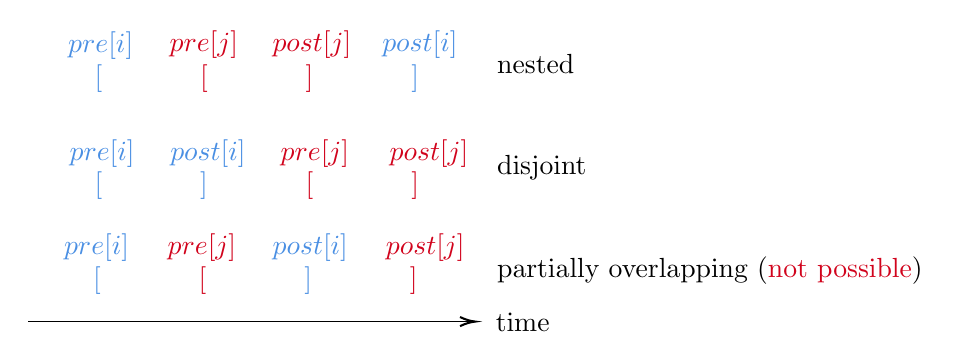
\begin{tikzpicture}[x=0.5pt,y=0.5pt,yscale=-1,xscale=1]
%uncomment if require: \path (0,295); %set diagram left start at 0, and has height of 295

%Straight Lines [id:da765632376076707] 
\draw    (32,273) -- (353,273) ;
\draw [shift={(355,273)}, rotate = 180] [color={rgb, 255:red, 0; green, 0; blue, 0 }  ][line width=0.75]    (10.93,-3.29) .. controls (6.95,-1.4) and (3.31,-0.3) .. (0,0) .. controls (3.31,0.3) and (6.95,1.4) .. (10.93,3.29)   ;

% Text Node
\draw (59,62) node [anchor=north west][inner sep=0.75pt]   [align=left] {$\displaystyle \textcolor[rgb]{0.29,0.56,0.89}{pre}\textcolor[rgb]{0.29,0.56,0.89}{[}\textcolor[rgb]{0.29,0.56,0.89}{i}\textcolor[rgb]{0.29,0.56,0.89}{]}$};
% Text Node
\draw (132.33,61) node [anchor=north west][inner sep=0.75pt]   [align=left] {$\displaystyle \textcolor[rgb]{0.82,0.01,0.11}{pre}\textcolor[rgb]{0.82,0.01,0.11}{[}\textcolor[rgb]{0.82,0.01,0.11}{j}\textcolor[rgb]{0.82,0.01,0.11}{]}$};
% Text Node
\draw (206.66,61) node [anchor=north west][inner sep=0.75pt]   [align=left] {$\displaystyle \textcolor[rgb]{0.82,0.01,0.11}{post}\textcolor[rgb]{0.82,0.01,0.11}{[}\textcolor[rgb]{0.82,0.01,0.11}{j}\textcolor[rgb]{0.82,0.01,0.11}{]}$};
% Text Node
\draw (286,61) node [anchor=north west][inner sep=0.75pt]   [align=left] {$\displaystyle \textcolor[rgb]{0.29,0.56,0.89}{post}\textcolor[rgb]{0.29,0.56,0.89}{[}\textcolor[rgb]{0.29,0.56,0.89}{i}\textcolor[rgb]{0.29,0.56,0.89}{]}$};
% Text Node
\draw (78,85.5) node [anchor=north west][inner sep=0.75pt]   [align=left] {$\displaystyle \textcolor[rgb]{0.29,0.56,0.89}{[}$};
% Text Node
\draw (154.33,85.5) node [anchor=north west][inner sep=0.75pt]   [align=left] {$\displaystyle \textcolor[rgb]{0.82,0.01,0.11}{[}$};
% Text Node
\draw (230.66,85.5) node [anchor=north west][inner sep=0.75pt]   [align=left] {$\displaystyle \textcolor[rgb]{0.82,0.01,0.11}{]}$};
% Text Node
\draw (307,85.5) node [anchor=north west][inner sep=0.75pt]   [align=left] {$\displaystyle \textcolor[rgb]{0.29,0.56,0.89}{]}$};
% Text Node
\draw (78,162.5) node [anchor=north west][inner sep=0.75pt]   [align=left] {$\displaystyle \textcolor[rgb]{0.29,0.56,0.89}{[}$};
% Text Node
\draw (154.33,162.5) node [anchor=north west][inner sep=0.75pt]   [align=left] {$\displaystyle \textcolor[rgb]{0.29,0.56,0.89}{]}$};
% Text Node
\draw (230.66,162.5) node [anchor=north west][inner sep=0.75pt]   [align=left] {$\displaystyle \textcolor[rgb]{0.82,0.01,0.11}{[}$};
% Text Node
\draw (307,162.5) node [anchor=north west][inner sep=0.75pt]   [align=left] {$\displaystyle \textcolor[rgb]{0.82,0.01,0.11}{]}$};
% Text Node
\draw (77,231.5) node [anchor=north west][inner sep=0.75pt]   [align=left] {$\displaystyle \textcolor[rgb]{0.29,0.56,0.89}{[}$};
% Text Node
\draw (153.33,231.5) node [anchor=north west][inner sep=0.75pt]   [align=left] {$\displaystyle \textcolor[rgb]{0.82,0.01,0.11}{[}$};
% Text Node
\draw (229.66,231.5) node [anchor=north west][inner sep=0.75pt]   [align=left] {$\displaystyle \textcolor[rgb]{0.29,0.56,0.89}{]}$};
% Text Node
\draw (306,231.5) node [anchor=north west][inner sep=0.75pt]   [align=left] {$\displaystyle \textcolor[rgb]{0.82,0.01,0.11}{]}$};
% Text Node
\draw (60,139.5) node [anchor=north west][inner sep=0.75pt]   [align=left] {$\displaystyle \textcolor[rgb]{0.29,0.56,0.89}{pre}\textcolor[rgb]{0.29,0.56,0.89}{[}\textcolor[rgb]{0.29,0.56,0.89}{i}\textcolor[rgb]{0.29,0.56,0.89}{]}$};
% Text Node
\draw (291.33,139.5) node [anchor=north west][inner sep=0.75pt]   [align=left] {$\displaystyle \textcolor[rgb]{0.82,0.01,0.11}{post}\textcolor[rgb]{0.82,0.01,0.11}{[}\textcolor[rgb]{0.82,0.01,0.11}{j}\textcolor[rgb]{0.82,0.01,0.11}{]}$};
% Text Node
\draw (212.56,139.5) node [anchor=north west][inner sep=0.75pt]   [align=left] {$\displaystyle \textcolor[rgb]{0.82,0.01,0.11}{pre}\textcolor[rgb]{0.82,0.01,0.11}{[}\textcolor[rgb]{0.82,0.01,0.11}{j}\textcolor[rgb]{0.82,0.01,0.11}{]}$};
% Text Node
\draw (132.78,139.5) node [anchor=north west][inner sep=0.75pt]   [align=left] {$\displaystyle \textcolor[rgb]{0.29,0.56,0.89}{post}\textcolor[rgb]{0.29,0.56,0.89}{[}\textcolor[rgb]{0.29,0.56,0.89}{i}\textcolor[rgb]{0.29,0.56,0.89}{]}$};
% Text Node
\draw (56,207.5) node [anchor=north west][inner sep=0.75pt]   [align=left] {$\displaystyle \textcolor[rgb]{0.29,0.56,0.89}{pre}\textcolor[rgb]{0.29,0.56,0.89}{[}\textcolor[rgb]{0.29,0.56,0.89}{i}\textcolor[rgb]{0.29,0.56,0.89}{]}$};
% Text Node
\draw (130.89,207.5) node [anchor=north west][inner sep=0.75pt]   [align=left] {$\displaystyle \textcolor[rgb]{0.82,0.01,0.11}{pre}\textcolor[rgb]{0.82,0.01,0.11}{[}\textcolor[rgb]{0.82,0.01,0.11}{j}\textcolor[rgb]{0.82,0.01,0.11}{]}$};
% Text Node
\draw (288.66,207.5) node [anchor=north west][inner sep=0.75pt]   [align=left] {$\displaystyle \textcolor[rgb]{0.82,0.01,0.11}{post}\textcolor[rgb]{0.82,0.01,0.11}{[}\textcolor[rgb]{0.82,0.01,0.11}{j}\textcolor[rgb]{0.82,0.01,0.11}{]}$};
% Text Node
\draw (206.78,207.5) node [anchor=north west][inner sep=0.75pt]   [align=left] {$\displaystyle \textcolor[rgb]{0.29,0.56,0.89}{post}\textcolor[rgb]{0.29,0.56,0.89}{[}\textcolor[rgb]{0.29,0.56,0.89}{i}\textcolor[rgb]{0.29,0.56,0.89}{]}$};
% Text Node
\draw (368,265) node [anchor=north west][inner sep=0.75pt]   [align=left] {time};
% Text Node
\draw (369,78) node [anchor=north west][inner sep=0.75pt]   [align=left] {nested};
% Text Node
\draw (369,151) node [anchor=north west][inner sep=0.75pt]   [align=left] {disjoint};
% Text Node
\draw (369,224) node [anchor=north west][inner sep=0.75pt]   [align=left] {partially overlapping (\textcolor[rgb]{0.82,0.01,0.11}{not possible})};


\end{tikzpicture}

}
\caption{Relations between two $[pre,post]$ intervals.}
\label{fig:interval}
\end{figure}

We now show and prove a key claim that relates the post values and the meta-graph.

\begin{claim}
Let $C_i$ and $C_j$ be two connected components of directed graph $G = (V, E)$, i.e., $C_i$ and $C_j$ are two
vertices in its coresponding meta-graph $G_M = (V_M, E_M)$. If we have $(C_i, C_j) \in E_M$ then
we must have that $\max_{u\in C_i} post[u] > \max_{v\in C_j} post[v]$.
\end{claim}

Intuitively, following an edge in the meta-graph, the largest post value decreases.
Before seeing a formal proof, please see an example in Figure~\ref{fig:dfs}:
the largest post values for $C_1$, $C_2$, $C_3$, and $C_4$ are 9, 6, 10, and 14,
and you may verify that following any edge in the meta-graph, the largest post value always decreases.

\begin{figure}[h!]
\centering{

\tikzset{every picture/.style={line width=0.75pt}} %set default line width to 0.75pt        

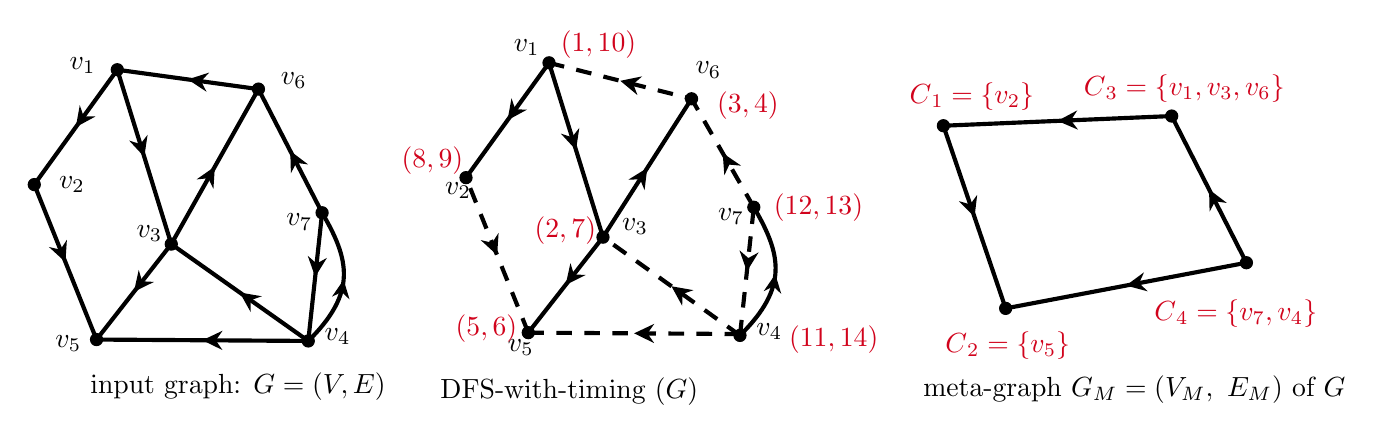
\begin{tikzpicture}[x=0.5pt,y=0.5pt,yscale=-1,xscale=1]
%uncomment if require: \path (0,284); %set diagram left start at 0, and has height of 284

%Flowchart: Connector [id:dp6832651596189389] 
\draw  [fill={rgb, 255:red, 0; green, 0; blue, 0 }  ,fill opacity=1 ] (69,40) .. controls (69,37.58) and (70.96,35.62) .. (73.38,35.62) .. controls (75.79,35.62) and (77.75,37.58) .. (77.75,40) .. controls (77.75,42.42) and (75.79,44.38) .. (73.38,44.38) .. controls (70.96,44.38) and (69,42.42) .. (69,40) -- cycle ;
%Flowchart: Connector [id:dp988004110095194] 
\draw  [fill={rgb, 255:red, 0; green, 0; blue, 0 }  ,fill opacity=1 ] (171,54) .. controls (171,51.58) and (172.96,49.62) .. (175.38,49.62) .. controls (177.79,49.62) and (179.75,51.58) .. (179.75,54) .. controls (179.75,56.42) and (177.79,58.38) .. (175.38,58.38) .. controls (172.96,58.38) and (171,56.42) .. (171,54) -- cycle ;
%Flowchart: Connector [id:dp8337455886193567] 
\draw  [fill={rgb, 255:red, 0; green, 0; blue, 0 }  ,fill opacity=1 ] (54,235) .. controls (54,232.58) and (55.96,230.62) .. (58.38,230.62) .. controls (60.79,230.62) and (62.75,232.58) .. (62.75,235) .. controls (62.75,237.42) and (60.79,239.38) .. (58.38,239.38) .. controls (55.96,239.38) and (54,237.42) .. (54,235) -- cycle ;
%Flowchart: Connector [id:dp7811656748056538] 
\draw  [fill={rgb, 255:red, 0; green, 0; blue, 0 }  ,fill opacity=1 ] (9,123) .. controls (9,120.58) and (10.96,118.62) .. (13.38,118.62) .. controls (15.79,118.62) and (17.75,120.58) .. (17.75,123) .. controls (17.75,125.42) and (15.79,127.38) .. (13.38,127.38) .. controls (10.96,127.38) and (9,125.42) .. (9,123) -- cycle ;
%Flowchart: Connector [id:dp7718177083818322] 
\draw  [fill={rgb, 255:red, 0; green, 0; blue, 0 }  ,fill opacity=1 ] (108,166) .. controls (108,163.58) and (109.96,161.62) .. (112.38,161.62) .. controls (114.79,161.62) and (116.75,163.58) .. (116.75,166) .. controls (116.75,168.42) and (114.79,170.38) .. (112.38,170.38) .. controls (109.96,170.38) and (108,168.42) .. (108,166) -- cycle ;
%Straight Lines [id:da8695282378045819] 
\draw [color={rgb, 255:red, 0; green, 0; blue, 0 }  ,draw opacity=1 ][line width=1.5]    (13.38,123) -- (73.38,40) ;
\draw [shift={(43.38,81.5)}, rotate = 305.86] [fill={rgb, 255:red, 0; green, 0; blue, 0 }  ,fill opacity=1 ][line width=0.08]  [draw opacity=0] (14.56,-6.99) -- (0,0) -- (14.56,6.99) -- (9.67,0) -- cycle    ;
%Straight Lines [id:da6240808629687105] 
\draw [color={rgb, 255:red, 0; green, 0; blue, 0 }  ,draw opacity=1 ][line width=1.5]    (58.38,235) -- (112.38,166) ;
\draw [shift={(85.38,200.5)}, rotate = 308.05] [fill={rgb, 255:red, 0; green, 0; blue, 0 }  ,fill opacity=1 ][line width=0.08]  [draw opacity=0] (14.56,-6.99) -- (0,0) -- (14.56,6.99) -- (9.67,0) -- cycle    ;
%Straight Lines [id:da28647521139148635] 
\draw [color={rgb, 255:red, 0; green, 0; blue, 0 }  ,draw opacity=1 ][line width=1.5]    (112.38,166) -- (73.38,40) ;
\draw [shift={(92.88,103)}, rotate = 252.8] [fill={rgb, 255:red, 0; green, 0; blue, 0 }  ,fill opacity=1 ][line width=0.08]  [draw opacity=0] (14.56,-6.99) -- (0,0) -- (14.56,6.99) -- (9.67,0) -- cycle    ;
%Straight Lines [id:da812435735905686] 
\draw [color={rgb, 255:red, 0; green, 0; blue, 0 }  ,draw opacity=1 ][line width=1.5]    (58.38,235) -- (13.38,123) ;
\draw [shift={(35.88,179)}, rotate = 248.11] [fill={rgb, 255:red, 0; green, 0; blue, 0 }  ,fill opacity=1 ][line width=0.08]  [draw opacity=0] (14.56,-6.99) -- (0,0) -- (14.56,6.99) -- (9.67,0) -- cycle    ;
%Flowchart: Connector [id:dp7779596833842585] 
\draw  [fill={rgb, 255:red, 0; green, 0; blue, 0 }  ,fill opacity=1 ] (207,236) .. controls (207,233.58) and (208.96,231.62) .. (211.38,231.62) .. controls (213.79,231.62) and (215.75,233.58) .. (215.75,236) .. controls (215.75,238.42) and (213.79,240.38) .. (211.38,240.38) .. controls (208.96,240.38) and (207,238.42) .. (207,236) -- cycle ;
%Straight Lines [id:da5661346124899681] 
\draw [color={rgb, 255:red, 0; green, 0; blue, 0 }  ,draw opacity=1 ][line width=1.5]    (211.38,236) -- (112.38,166) ;
\draw [shift={(161.88,201)}, rotate = 395.26] [fill={rgb, 255:red, 0; green, 0; blue, 0 }  ,fill opacity=1 ][line width=0.08]  [draw opacity=0] (14.56,-6.99) -- (0,0) -- (14.56,6.99) -- (9.67,0) -- cycle    ;
%Straight Lines [id:da9652070356210863] 
\draw [color={rgb, 255:red, 0; green, 0; blue, 0 }  ,draw opacity=1 ][line width=1.5]    (58.38,235) -- (211.38,236) ;
\draw [shift={(134.88,235.5)}, rotate = 0.37] [fill={rgb, 255:red, 0; green, 0; blue, 0 }  ,fill opacity=1 ][line width=0.08]  [draw opacity=0] (14.56,-6.99) -- (0,0) -- (14.56,6.99) -- (9.67,0) -- cycle    ;
%Flowchart: Connector [id:dp27050103826240035] 
\draw  [fill={rgb, 255:red, 0; green, 0; blue, 0 }  ,fill opacity=1 ] (217,143.38) .. controls (217,140.96) and (218.96,139) .. (221.38,139) .. controls (223.79,139) and (225.75,140.96) .. (225.75,143.38) .. controls (225.75,145.79) and (223.79,147.75) .. (221.38,147.75) .. controls (218.96,147.75) and (217,145.79) .. (217,143.38) -- cycle ;
%Straight Lines [id:da42141438650125873] 
\draw [color={rgb, 255:red, 0; green, 0; blue, 0 }  ,draw opacity=1 ][line width=1.5]    (221.38,143.38) -- (175.38,54) ;
\draw [shift={(198.38,98.69)}, rotate = 422.77] [fill={rgb, 255:red, 0; green, 0; blue, 0 }  ,fill opacity=1 ][line width=0.08]  [draw opacity=0] (14.56,-6.99) -- (0,0) -- (14.56,6.99) -- (9.67,0) -- cycle    ;
%Flowchart: Connector [id:dp9280107639837872] 
\draw  [fill={rgb, 255:red, 0; green, 0; blue, 0 }  ,fill opacity=1 ] (381,35) .. controls (381,32.58) and (382.96,30.62) .. (385.38,30.62) .. controls (387.79,30.62) and (389.75,32.58) .. (389.75,35) .. controls (389.75,37.42) and (387.79,39.38) .. (385.38,39.38) .. controls (382.96,39.38) and (381,37.42) .. (381,35) -- cycle ;
%Flowchart: Connector [id:dp32325565860173133] 
\draw  [fill={rgb, 255:red, 0; green, 0; blue, 0 }  ,fill opacity=1 ] (366,230) .. controls (366,227.58) and (367.96,225.62) .. (370.38,225.62) .. controls (372.79,225.62) and (374.75,227.58) .. (374.75,230) .. controls (374.75,232.42) and (372.79,234.38) .. (370.38,234.38) .. controls (367.96,234.38) and (366,232.42) .. (366,230) -- cycle ;
%Flowchart: Connector [id:dp9891123981062072] 
\draw  [fill={rgb, 255:red, 0; green, 0; blue, 0 }  ,fill opacity=1 ] (321,118) .. controls (321,115.58) and (322.96,113.62) .. (325.38,113.62) .. controls (327.79,113.62) and (329.75,115.58) .. (329.75,118) .. controls (329.75,120.42) and (327.79,122.38) .. (325.38,122.38) .. controls (322.96,122.38) and (321,120.42) .. (321,118) -- cycle ;
%Flowchart: Connector [id:dp40112220553719025] 
\draw  [fill={rgb, 255:red, 0; green, 0; blue, 0 }  ,fill opacity=1 ] (420,161) .. controls (420,158.58) and (421.96,156.62) .. (424.38,156.62) .. controls (426.79,156.62) and (428.75,158.58) .. (428.75,161) .. controls (428.75,163.42) and (426.79,165.38) .. (424.38,165.38) .. controls (421.96,165.38) and (420,163.42) .. (420,161) -- cycle ;
%Straight Lines [id:da23221470279057188] 
\draw [color={rgb, 255:red, 0; green, 0; blue, 0 }  ,draw opacity=1 ][line width=1.5]    (325.38,118) -- (385.38,35) ;
\draw [shift={(355.38,76.5)}, rotate = 305.86] [fill={rgb, 255:red, 0; green, 0; blue, 0 }  ,fill opacity=1 ][line width=0.08]  [draw opacity=0] (14.56,-6.99) -- (0,0) -- (14.56,6.99) -- (9.67,0) -- cycle    ;
%Straight Lines [id:da9690767143154184] 
\draw [color={rgb, 255:red, 0; green, 0; blue, 0 }  ,draw opacity=1 ][line width=1.5]  [dash pattern={on 5.63pt off 4.5pt}]  (370.38,230) -- (325.38,118) ;
\draw [shift={(347.88,174)}, rotate = 248.11] [fill={rgb, 255:red, 0; green, 0; blue, 0 }  ,fill opacity=1 ][line width=0.08]  [draw opacity=0] (14.56,-6.99) -- (0,0) -- (14.56,6.99) -- (9.67,0) -- cycle    ;
%Straight Lines [id:da5442772122834477] 
\draw [color={rgb, 255:red, 0; green, 0; blue, 0 }  ,draw opacity=1 ][line width=1.5]    (112.38,166) -- (175.38,54) ;
\draw [shift={(143.88,110)}, rotate = 479.36] [fill={rgb, 255:red, 0; green, 0; blue, 0 }  ,fill opacity=1 ][line width=0.08]  [draw opacity=0] (14.56,-6.99) -- (0,0) -- (14.56,6.99) -- (9.67,0) -- cycle    ;
%Straight Lines [id:da054951132315465334] 
\draw [color={rgb, 255:red, 0; green, 0; blue, 0 }  ,draw opacity=1 ][line width=1.5]    (73.38,40) -- (175.38,54) ;
\draw [shift={(124.38,47)}, rotate = 7.82] [fill={rgb, 255:red, 0; green, 0; blue, 0 }  ,fill opacity=1 ][line width=0.08]  [draw opacity=0] (14.56,-6.99) -- (0,0) -- (14.56,6.99) -- (9.67,0) -- cycle    ;
%Straight Lines [id:da4714865771303105] 
\draw [color={rgb, 255:red, 0; green, 0; blue, 0 }  ,draw opacity=1 ][line width=1.5]    (211.38,236) -- (221.38,143.38) ;
\draw [shift={(216.38,189.69)}, rotate = 276.16] [fill={rgb, 255:red, 0; green, 0; blue, 0 }  ,fill opacity=1 ][line width=0.08]  [draw opacity=0] (14.56,-6.99) -- (0,0) -- (14.56,6.99) -- (9.67,0) -- cycle    ;
%Flowchart: Connector [id:dp8072873078420509] 
\draw  [fill={rgb, 255:red, 0; green, 0; blue, 0 }  ,fill opacity=1 ] (484,61) .. controls (484,58.58) and (485.96,56.62) .. (488.38,56.62) .. controls (490.79,56.62) and (492.75,58.58) .. (492.75,61) .. controls (492.75,63.42) and (490.79,65.38) .. (488.38,65.38) .. controls (485.96,65.38) and (484,63.42) .. (484,61) -- cycle ;
%Straight Lines [id:da8862996829120494] 
\draw [color={rgb, 255:red, 0; green, 0; blue, 0 }  ,draw opacity=1 ][line width=1.5]    (424.38,161) -- (385.38,35) ;
\draw [shift={(404.88,98)}, rotate = 252.8] [fill={rgb, 255:red, 0; green, 0; blue, 0 }  ,fill opacity=1 ][line width=0.08]  [draw opacity=0] (14.56,-6.99) -- (0,0) -- (14.56,6.99) -- (9.67,0) -- cycle    ;
%Straight Lines [id:da8175209497677637] 
\draw [color={rgb, 255:red, 0; green, 0; blue, 0 }  ,draw opacity=1 ][line width=1.5]    (370.38,230) -- (424.38,161) ;
\draw [shift={(397.38,195.5)}, rotate = 308.05] [fill={rgb, 255:red, 0; green, 0; blue, 0 }  ,fill opacity=1 ][line width=0.08]  [draw opacity=0] (14.56,-6.99) -- (0,0) -- (14.56,6.99) -- (9.67,0) -- cycle    ;
%Straight Lines [id:da4545876322404935] 
\draw [color={rgb, 255:red, 0; green, 0; blue, 0 }  ,draw opacity=1 ][line width=1.5]    (488.38,61) -- (424.38,161) ;
\draw [shift={(456.38,111)}, rotate = 122.62] [fill={rgb, 255:red, 0; green, 0; blue, 0 }  ,fill opacity=1 ][line width=0.08]  [draw opacity=0] (14.56,-6.99) -- (0,0) -- (14.56,6.99) -- (9.67,0) -- cycle    ;
%Straight Lines [id:da2228311257049178] 
\draw [color={rgb, 255:red, 0; green, 0; blue, 0 }  ,draw opacity=1 ][line width=1.5]  [dash pattern={on 5.63pt off 4.5pt}]  (385.38,35) -- (488.38,61) ;
\draw [shift={(436.88,48)}, rotate = 14.17] [fill={rgb, 255:red, 0; green, 0; blue, 0 }  ,fill opacity=1 ][line width=0.08]  [draw opacity=0] (14.56,-6.99) -- (0,0) -- (14.56,6.99) -- (9.67,0) -- cycle    ;
%Flowchart: Connector [id:dp13927282273128694] 
\draw  [fill={rgb, 255:red, 0; green, 0; blue, 0 }  ,fill opacity=1 ] (519,232) .. controls (519,229.58) and (520.96,227.62) .. (523.38,227.62) .. controls (525.79,227.62) and (527.75,229.58) .. (527.75,232) .. controls (527.75,234.42) and (525.79,236.38) .. (523.38,236.38) .. controls (520.96,236.38) and (519,234.42) .. (519,232) -- cycle ;
%Straight Lines [id:da9522823837992999] 
\draw [color={rgb, 255:red, 0; green, 0; blue, 0 }  ,draw opacity=1 ][line width=1.5]  [dash pattern={on 5.63pt off 4.5pt}]  (523.38,232) -- (424.38,161) ;
\draw [shift={(473.88,196.5)}, rotate = 395.65] [fill={rgb, 255:red, 0; green, 0; blue, 0 }  ,fill opacity=1 ][line width=0.08]  [draw opacity=0] (14.56,-6.99) -- (0,0) -- (14.56,6.99) -- (9.67,0) -- cycle    ;
%Straight Lines [id:da9451785250835093] 
\draw [color={rgb, 255:red, 0; green, 0; blue, 0 }  ,draw opacity=1 ][line width=1.5]  [dash pattern={on 5.63pt off 4.5pt}]  (370.38,230) -- (523.38,231) ;
\draw [shift={(446.88,230.5)}, rotate = 0.37] [fill={rgb, 255:red, 0; green, 0; blue, 0 }  ,fill opacity=1 ][line width=0.08]  [draw opacity=0] (14.56,-6.99) -- (0,0) -- (14.56,6.99) -- (9.67,0) -- cycle    ;
%Flowchart: Connector [id:dp6205422729267549] 
\draw  [fill={rgb, 255:red, 0; green, 0; blue, 0 }  ,fill opacity=1 ] (529,139.38) .. controls (529,136.96) and (530.96,135) .. (533.38,135) .. controls (535.79,135) and (537.75,136.96) .. (537.75,139.38) .. controls (537.75,141.79) and (535.79,143.75) .. (533.38,143.75) .. controls (530.96,143.75) and (529,141.79) .. (529,139.38) -- cycle ;
%Straight Lines [id:da8040330863088329] 
\draw [color={rgb, 255:red, 0; green, 0; blue, 0 }  ,draw opacity=1 ][line width=1.5]  [dash pattern={on 5.63pt off 4.5pt}]  (533.38,139.38) -- (488.38,61) ;
\draw [shift={(510.88,100.19)}, rotate = 420.14] [fill={rgb, 255:red, 0; green, 0; blue, 0 }  ,fill opacity=1 ][line width=0.08]  [draw opacity=0] (14.56,-6.99) -- (0,0) -- (14.56,6.99) -- (9.67,0) -- cycle    ;
%Straight Lines [id:da270721811462559] 
\draw [color={rgb, 255:red, 0; green, 0; blue, 0 }  ,draw opacity=1 ][line width=1.5]  [dash pattern={on 5.63pt off 4.5pt}]  (523.38,232) -- (533.38,139.38) ;
\draw [shift={(528.38,185.69)}, rotate = 276.16] [fill={rgb, 255:red, 0; green, 0; blue, 0 }  ,fill opacity=1 ][line width=0.08]  [draw opacity=0] (14.56,-6.99) -- (0,0) -- (14.56,6.99) -- (9.67,0) -- cycle    ;
%Curve Lines [id:da3335117221128735] 
\draw [line width=1.5]    (211.38,236) .. controls (247,201) and (241,177) .. (221.38,143.38) ;
\draw [shift={(236.93,191.8)}, rotate = 458.86] [fill={rgb, 255:red, 0; green, 0; blue, 0 }  ][line width=0.08]  [draw opacity=0] (13.4,-6.43) -- (0,0) -- (13.4,6.44) -- (8.9,0) -- cycle    ;
%Curve Lines [id:da3048800924799854] 
\draw [line width=1.5]    (523.38,232) .. controls (559,197) and (553,173) .. (533.38,139.38) ;
\draw [shift={(548.93,187.8)}, rotate = 458.86] [fill={rgb, 255:red, 0; green, 0; blue, 0 }  ][line width=0.08]  [draw opacity=0] (13.4,-6.43) -- (0,0) -- (13.4,6.44) -- (8.9,0) -- cycle    ;
%Flowchart: Connector [id:dp4802213327188575] 
\draw  [fill={rgb, 255:red, 0; green, 0; blue, 0 }  ,fill opacity=1 ] (711,212.47) .. controls (711,210.05) and (712.96,208.09) .. (715.38,208.09) .. controls (717.79,208.09) and (719.75,210.05) .. (719.75,212.47) .. controls (719.75,214.89) and (717.79,216.85) .. (715.38,216.85) .. controls (712.96,216.85) and (711,214.89) .. (711,212.47) -- cycle ;
%Straight Lines [id:da4012018667347226] 
\draw [color={rgb, 255:red, 0; green, 0; blue, 0 }  ,draw opacity=1 ][line width=1.5]    (889.38,179.47) -- (835.38,73.47) ;
\draw [shift={(862.38,126.47)}, rotate = 423] [fill={rgb, 255:red, 0; green, 0; blue, 0 }  ,fill opacity=1 ][line width=0.08]  [draw opacity=0] (14.56,-6.99) -- (0,0) -- (14.56,6.99) -- (9.67,0) -- cycle    ;
%Flowchart: Connector [id:dp8765246990395692] 
\draw  [fill={rgb, 255:red, 0; green, 0; blue, 0 }  ,fill opacity=1 ] (831,73.47) .. controls (831,71.05) and (832.96,69.09) .. (835.38,69.09) .. controls (837.79,69.09) and (839.75,71.05) .. (839.75,73.47) .. controls (839.75,75.89) and (837.79,77.85) .. (835.38,77.85) .. controls (832.96,77.85) and (831,75.89) .. (831,73.47) -- cycle ;
%Flowchart: Connector [id:dp16478045407286646] 
\draw  [fill={rgb, 255:red, 0; green, 0; blue, 0 }  ,fill opacity=1 ] (666,80.47) .. controls (666,78.05) and (667.96,76.09) .. (670.38,76.09) .. controls (672.79,76.09) and (674.75,78.05) .. (674.75,80.47) .. controls (674.75,82.89) and (672.79,84.85) .. (670.38,84.85) .. controls (667.96,84.85) and (666,82.89) .. (666,80.47) -- cycle ;
%Straight Lines [id:da43610676953677097] 
\draw [color={rgb, 255:red, 0; green, 0; blue, 0 }  ,draw opacity=1 ][line width=1.5]    (715.38,212.47) -- (670.38,80.47) ;
\draw [shift={(692.88,146.47)}, rotate = 251.18] [fill={rgb, 255:red, 0; green, 0; blue, 0 }  ,fill opacity=1 ][line width=0.08]  [draw opacity=0] (14.56,-6.99) -- (0,0) -- (14.56,6.99) -- (9.67,0) -- cycle    ;
%Straight Lines [id:da9496215087963258] 
\draw [color={rgb, 255:red, 0; green, 0; blue, 0 }  ,draw opacity=1 ][line width=1.5]    (670.38,80.47) -- (835.38,73.47) ;
\draw [shift={(752.88,76.97)}, rotate = 357.57] [fill={rgb, 255:red, 0; green, 0; blue, 0 }  ,fill opacity=1 ][line width=0.08]  [draw opacity=0] (14.56,-6.99) -- (0,0) -- (14.56,6.99) -- (9.67,0) -- cycle    ;
%Flowchart: Connector [id:dp3010893945707027] 
\draw  [fill={rgb, 255:red, 0; green, 0; blue, 0 }  ,fill opacity=1 ] (885,179.47) .. controls (885,177.05) and (886.96,175.09) .. (889.38,175.09) .. controls (891.79,175.09) and (893.75,177.05) .. (893.75,179.47) .. controls (893.75,181.89) and (891.79,183.85) .. (889.38,183.85) .. controls (886.96,183.85) and (885,181.89) .. (885,179.47) -- cycle ;
%Straight Lines [id:da25219897920368006] 
\draw [color={rgb, 255:red, 0; green, 0; blue, 0 }  ,draw opacity=1 ][line width=1.5]    (889.38,179.47) -- (715.38,212.47) ;
\draw [shift={(802.38,195.97)}, rotate = 349.26] [fill={rgb, 255:red, 0; green, 0; blue, 0 }  ,fill opacity=1 ][line width=0.08]  [draw opacity=0] (14.56,-6.99) -- (0,0) -- (14.56,6.99) -- (9.67,0) -- cycle    ;

% Text Node
\draw (37,29) node [anchor=north west][inner sep=0.75pt]   [align=left] {$\displaystyle v_{1}$};
% Text Node
\draw (85.38,150.38) node [anchor=north west][inner sep=0.75pt]   [align=left] {$\displaystyle v_{3}$};
% Text Node
\draw (26.75,230) node [anchor=north west][inner sep=0.75pt]   [align=left] {$\displaystyle v_{5}$};
% Text Node
\draw (221.38,225.38) node [anchor=north west][inner sep=0.75pt]   [align=left] {$\displaystyle v_{4}$};
% Text Node
\draw (29.38,115.38) node [anchor=north west][inner sep=0.75pt]   [align=left] {$\displaystyle v_{2}$};
% Text Node
\draw (189.75,40.35) node [anchor=north west][inner sep=0.75pt]   [align=left] {$\displaystyle v_{6}$};
% Text Node
\draw (193.75,142.35) node [anchor=north west][inner sep=0.75pt]   [align=left] {$\displaystyle v_{7}$};
% Text Node
\draw (52,256.93) node [anchor=north west][inner sep=0.75pt]   [align=left] {input graph: $\displaystyle G=( V,E)$};
% Text Node
\draw (358,16) node [anchor=north west][inner sep=0.75pt]   [align=left] {$\displaystyle v_{1}$};
% Text Node
\draw (436.38,145.38) node [anchor=north west][inner sep=0.75pt]   [align=left] {$\displaystyle v_{3}$};
% Text Node
\draw (353.75,233) node [anchor=north west][inner sep=0.75pt]   [align=left] {$\displaystyle v_{5}$};
% Text Node
\draw (308.38,119.38) node [anchor=north west][inner sep=0.75pt]   [align=left] {$\displaystyle v_{2}$};
% Text Node
\draw (305,260.93) node [anchor=north west][inner sep=0.75pt]   [align=left] {DFS-with-timing~$\displaystyle(G)$};
% Text Node
\draw (489.38,32.48) node [anchor=north west][inner sep=0.75pt]   [align=left] {$\displaystyle v_{6}$};
% Text Node
\draw (533.38,221.38) node [anchor=north west][inner sep=0.75pt]   [align=left] {$\displaystyle v_{4}$};
% Text Node
\draw (505.75,138.35) node [anchor=north west][inner sep=0.75pt]   [align=left] {$\displaystyle v_{7}$};
% Text Node
\draw (392,10) node [anchor=north west][inner sep=0.75pt]   [align=left] {$\displaystyle \textcolor[rgb]{0.82,0.01,0.11}{(}\textcolor[rgb]{0.82,0.01,0.11}{1,10}\textcolor[rgb]{0.82,0.01,0.11}{)}$};
% Text Node
\draw (277,94) node [anchor=north west][inner sep=0.75pt]   [align=left] {$\displaystyle \textcolor[rgb]{0.82,0.01,0.11}{(}\textcolor[rgb]{0.82,0.01,0.11}{8,9}\textcolor[rgb]{0.82,0.01,0.11}{)}$};
% Text Node
\draw (316,215) node [anchor=north west][inner sep=0.75pt]   [align=left] {$\displaystyle \textcolor[rgb]{0.82,0.01,0.11}{(}\textcolor[rgb]{0.82,0.01,0.11}{5,6}\textcolor[rgb]{0.82,0.01,0.11}{)}$};
% Text Node
\draw (373,144) node [anchor=north west][inner sep=0.75pt]   [align=left] {$\displaystyle \textcolor[rgb]{0.82,0.01,0.11}{(}\textcolor[rgb]{0.82,0.01,0.11}{2,7}\textcolor[rgb]{0.82,0.01,0.11}{)}$};
% Text Node
\draw (546,128) node [anchor=north west][inner sep=0.75pt]   [align=left] {$\displaystyle \textcolor[rgb]{0.82,0.01,0.11}{(}\textcolor[rgb]{0.82,0.01,0.11}{12,13}\textcolor[rgb]{0.82,0.01,0.11}{)}$};
% Text Node
\draw (505,54) node [anchor=north west][inner sep=0.75pt]   [align=left] {$\displaystyle \textcolor[rgb]{0.82,0.01,0.11}{(}\textcolor[rgb]{0.82,0.01,0.11}{3,4}\textcolor[rgb]{0.82,0.01,0.11}{)}$};
% Text Node
\draw (557,223) node [anchor=north west][inner sep=0.75pt]   [align=left] {$\displaystyle \textcolor[rgb]{0.82,0.01,0.11}{(}\textcolor[rgb]{0.82,0.01,0.11}{11,14}\textcolor[rgb]{0.82,0.01,0.11}{)}$};
% Text Node
\draw (670,227.47) node [anchor=north west][inner sep=0.75pt]   [align=left] {$\displaystyle \textcolor[rgb]{0.82,0.01,0.11}{C}\textcolor[rgb]{0.82,0.01,0.11}{_{2} =\{v_{5}\}}$};
% Text Node
\draw (821,204.47) node [anchor=north west][inner sep=0.75pt]   [align=left] {$\displaystyle \textcolor[rgb]{0.82,0.01,0.11}{C}\textcolor[rgb]{0.82,0.01,0.11}{_{4} =\{v_{7} ,v_{4}\}}$};
% Text Node
\draw (644,47.47) node [anchor=north west][inner sep=0.75pt]   [align=left] {$\displaystyle \textcolor[rgb]{0.82,0.01,0.11}{C}\textcolor[rgb]{0.82,0.01,0.11}{_{1} =\{v_{2}\}}$};
% Text Node
\draw (770,41.47) node [anchor=north west][inner sep=0.75pt]   [align=left] {$\displaystyle \textcolor[rgb]{0.82,0.01,0.11}{C}\textcolor[rgb]{0.82,0.01,0.11}{_{3} =\{v_{1} ,v_{3} ,v_{6}\}}$};
% Text Node
\draw (654,259.47) node [anchor=north west][inner sep=0.75pt]   [align=left] {meta-graph $\displaystyle G_{M} =( V_{M} ,\ E_{M})$ of $\displaystyle G$};


\end{tikzpicture}

}
\caption{Example of running DFS~(with timing) on a directed graph. The $[pre,post]$ interval for each vertex
is marked next to each vertex.  The $postlist$ for this run is \textcolor{blue}{$postlist = (v_4,v_7,v_1,v_2,v_3,v_5,v_6)$}.  }
\label{fig:dfs}
\end{figure}



\emph{Proof.} Let $u^* := \arg\min_{u\in C_i\cup C_j} pre[u]$, i.e., $u^*$ is the first explored vertex in $C_i\cup C_j$.
Consider the two cases. 

\begin{figure}[h!]
\centering{

\tikzset{every picture/.style={line width=0.75pt}} %set default line width to 0.75pt        

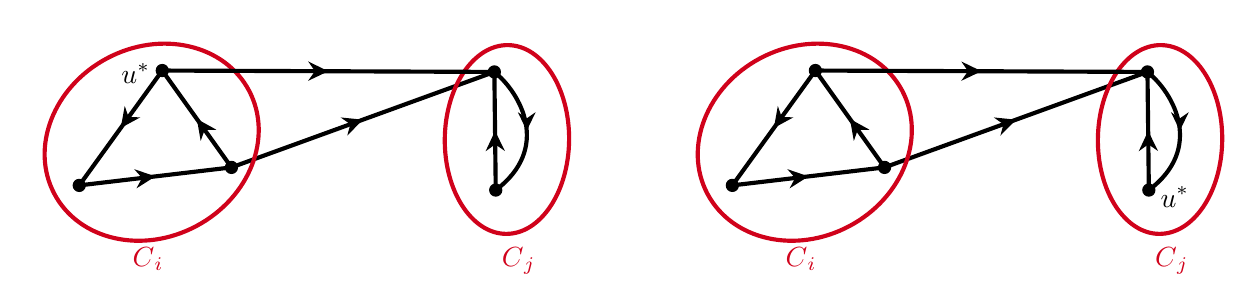
\begin{tikzpicture}[x=0.5pt,y=0.5pt,yscale=-1,xscale=1]
%uncomment if require: \path (0,196); %set diagram left start at 0, and has height of 196

%Flowchart: Connector [id:dp6536711043457765] 
\draw  [fill={rgb, 255:red, 0; green, 0; blue, 0 }  ,fill opacity=1 ] (92,42) .. controls (92,39.58) and (93.96,37.62) .. (96.38,37.62) .. controls (98.79,37.62) and (100.75,39.58) .. (100.75,42) .. controls (100.75,44.42) and (98.79,46.38) .. (96.38,46.38) .. controls (93.96,46.38) and (92,44.42) .. (92,42) -- cycle ;
%Flowchart: Connector [id:dp4048504811962438] 
\draw  [fill={rgb, 255:red, 0; green, 0; blue, 0 }  ,fill opacity=1 ] (32,125) .. controls (32,122.58) and (33.96,120.62) .. (36.38,120.62) .. controls (38.79,120.62) and (40.75,122.58) .. (40.75,125) .. controls (40.75,127.42) and (38.79,129.38) .. (36.38,129.38) .. controls (33.96,129.38) and (32,127.42) .. (32,125) -- cycle ;
%Flowchart: Connector [id:dp5803674133267218] 
\draw  [fill={rgb, 255:red, 0; green, 0; blue, 0 }  ,fill opacity=1 ] (142,112) .. controls (142,109.58) and (143.96,107.62) .. (146.38,107.62) .. controls (148.79,107.62) and (150.75,109.58) .. (150.75,112) .. controls (150.75,114.42) and (148.79,116.38) .. (146.38,116.38) .. controls (143.96,116.38) and (142,114.42) .. (142,112) -- cycle ;
%Straight Lines [id:da41352412753482715] 
\draw [color={rgb, 255:red, 0; green, 0; blue, 0 }  ,draw opacity=1 ][line width=1.5]    (36.38,125) -- (96.38,42) ;
\draw [shift={(66.38,83.5)}, rotate = 305.86] [fill={rgb, 255:red, 0; green, 0; blue, 0 }  ,fill opacity=1 ][line width=0.08]  [draw opacity=0] (14.56,-6.99) -- (0,0) -- (14.56,6.99) -- (9.67,0) -- cycle    ;
%Straight Lines [id:da10247422093058312] 
\draw [color={rgb, 255:red, 0; green, 0; blue, 0 }  ,draw opacity=1 ][line width=1.5]    (146.38,112) -- (36.38,125) ;
\draw [shift={(91.38,118.5)}, rotate = 173.26] [fill={rgb, 255:red, 0; green, 0; blue, 0 }  ,fill opacity=1 ][line width=0.08]  [draw opacity=0] (14.56,-6.99) -- (0,0) -- (14.56,6.99) -- (9.67,0) -- cycle    ;
%Flowchart: Connector [id:dp9895082549389806] 
\draw  [fill={rgb, 255:red, 0; green, 0; blue, 0 }  ,fill opacity=1 ] (333,128.38) .. controls (333,125.96) and (334.96,124) .. (337.38,124) .. controls (339.79,124) and (341.75,125.96) .. (341.75,128.38) .. controls (341.75,130.79) and (339.79,132.75) .. (337.38,132.75) .. controls (334.96,132.75) and (333,130.79) .. (333,128.38) -- cycle ;
%Straight Lines [id:da8137901366298937] 
\draw [color={rgb, 255:red, 0; green, 0; blue, 0 }  ,draw opacity=1 ][line width=1.5]    (337.38,128.38) -- (336.38,43) ;
\draw [shift={(336.88,85.69)}, rotate = 449.33] [fill={rgb, 255:red, 0; green, 0; blue, 0 }  ,fill opacity=1 ][line width=0.08]  [draw opacity=0] (14.56,-6.99) -- (0,0) -- (14.56,6.99) -- (9.67,0) -- cycle    ;
%Straight Lines [id:da15716373425720087] 
\draw [color={rgb, 255:red, 0; green, 0; blue, 0 }  ,draw opacity=1 ][line width=1.5]    (96.38,42) -- (146.38,112) ;
\draw [shift={(121.38,77)}, rotate = 54.46] [fill={rgb, 255:red, 0; green, 0; blue, 0 }  ,fill opacity=1 ][line width=0.08]  [draw opacity=0] (14.56,-6.99) -- (0,0) -- (14.56,6.99) -- (9.67,0) -- cycle    ;
%Flowchart: Connector [id:dp2761717414077073] 
\draw  [fill={rgb, 255:red, 0; green, 0; blue, 0 }  ,fill opacity=1 ] (332,43) .. controls (332,40.58) and (333.96,38.62) .. (336.38,38.62) .. controls (338.79,38.62) and (340.75,40.58) .. (340.75,43) .. controls (340.75,45.42) and (338.79,47.38) .. (336.38,47.38) .. controls (333.96,47.38) and (332,45.42) .. (332,43) -- cycle ;
%Curve Lines [id:da7005340985732622] 
\draw [line width=1.5]    (337.38,128.38) .. controls (377.38,98.38) and (355.68,58.52) .. (336.38,43) ;
\draw [shift={(359.77,85.48)}, rotate = 270.05] [fill={rgb, 255:red, 0; green, 0; blue, 0 }  ][line width=0.08]  [draw opacity=0] (13.4,-6.43) -- (0,0) -- (13.4,6.44) -- (8.9,0) -- cycle    ;
%Straight Lines [id:da9578319160914094] 
\draw [color={rgb, 255:red, 0; green, 0; blue, 0 }  ,draw opacity=1 ][line width=1.5]    (146.38,112) -- (336.38,43) ;
\draw [shift={(241.38,77.5)}, rotate = 520.04] [fill={rgb, 255:red, 0; green, 0; blue, 0 }  ,fill opacity=1 ][line width=0.08]  [draw opacity=0] (14.56,-6.99) -- (0,0) -- (14.56,6.99) -- (9.67,0) -- cycle    ;
%Shape: Ellipse [id:dp7130795758017592] 
\draw  [color={rgb, 255:red, 208; green, 2; blue, 27 }  ,draw opacity=1 ][line width=1.5]  (18.39,131.12) .. controls (0.61,97.62) and (17.68,53.75) .. (56.52,33.13) .. controls (95.37,12.52) and (141.27,22.96) .. (159.05,56.45) .. controls (176.83,89.95) and (159.76,133.82) .. (120.91,154.44) .. controls (82.07,175.06) and (36.17,164.61) .. (18.39,131.12) -- cycle ;
%Shape: Ellipse [id:dp3252588920876551] 
\draw  [color={rgb, 255:red, 208; green, 2; blue, 27 }  ,draw opacity=1 ][line width=1.5]  (346.2,23.61) .. controls (371.02,23.88) and (390.8,54.63) .. (390.4,92.31) .. controls (390,129.98) and (369.56,160.31) .. (344.75,160.04) .. controls (319.94,159.78) and (300.15,129.02) .. (300.55,91.35) .. controls (300.96,53.68) and (321.39,23.35) .. (346.2,23.61) -- cycle ;
%Straight Lines [id:da5477464737595377] 
\draw [color={rgb, 255:red, 0; green, 0; blue, 0 }  ,draw opacity=1 ][line width=1.5]    (96.38,42) -- (336.38,43) ;
\draw [shift={(216.38,42.5)}, rotate = 180.24] [fill={rgb, 255:red, 0; green, 0; blue, 0 }  ,fill opacity=1 ][line width=0.08]  [draw opacity=0] (14.56,-6.99) -- (0,0) -- (14.56,6.99) -- (9.67,0) -- cycle    ;
%Flowchart: Connector [id:dp1899602180220128] 
\draw  [fill={rgb, 255:red, 0; green, 0; blue, 0 }  ,fill opacity=1 ] (564,42) .. controls (564,39.58) and (565.96,37.62) .. (568.38,37.62) .. controls (570.79,37.62) and (572.75,39.58) .. (572.75,42) .. controls (572.75,44.42) and (570.79,46.38) .. (568.38,46.38) .. controls (565.96,46.38) and (564,44.42) .. (564,42) -- cycle ;
%Flowchart: Connector [id:dp3367645532097966] 
\draw  [fill={rgb, 255:red, 0; green, 0; blue, 0 }  ,fill opacity=1 ] (504,125) .. controls (504,122.58) and (505.96,120.62) .. (508.38,120.62) .. controls (510.79,120.62) and (512.75,122.58) .. (512.75,125) .. controls (512.75,127.42) and (510.79,129.38) .. (508.38,129.38) .. controls (505.96,129.38) and (504,127.42) .. (504,125) -- cycle ;
%Flowchart: Connector [id:dp1636605325292072] 
\draw  [fill={rgb, 255:red, 0; green, 0; blue, 0 }  ,fill opacity=1 ] (614,112) .. controls (614,109.58) and (615.96,107.62) .. (618.38,107.62) .. controls (620.79,107.62) and (622.75,109.58) .. (622.75,112) .. controls (622.75,114.42) and (620.79,116.38) .. (618.38,116.38) .. controls (615.96,116.38) and (614,114.42) .. (614,112) -- cycle ;
%Straight Lines [id:da7434793312503435] 
\draw [color={rgb, 255:red, 0; green, 0; blue, 0 }  ,draw opacity=1 ][line width=1.5]    (508.38,125) -- (568.38,42) ;
\draw [shift={(538.38,83.5)}, rotate = 305.86] [fill={rgb, 255:red, 0; green, 0; blue, 0 }  ,fill opacity=1 ][line width=0.08]  [draw opacity=0] (14.56,-6.99) -- (0,0) -- (14.56,6.99) -- (9.67,0) -- cycle    ;
%Straight Lines [id:da5706567229622709] 
\draw [color={rgb, 255:red, 0; green, 0; blue, 0 }  ,draw opacity=1 ][line width=1.5]    (618.38,112) -- (508.38,125) ;
\draw [shift={(563.38,118.5)}, rotate = 173.26] [fill={rgb, 255:red, 0; green, 0; blue, 0 }  ,fill opacity=1 ][line width=0.08]  [draw opacity=0] (14.56,-6.99) -- (0,0) -- (14.56,6.99) -- (9.67,0) -- cycle    ;
%Flowchart: Connector [id:dp05787420135544841] 
\draw  [fill={rgb, 255:red, 0; green, 0; blue, 0 }  ,fill opacity=1 ] (805,128.38) .. controls (805,125.96) and (806.96,124) .. (809.38,124) .. controls (811.79,124) and (813.75,125.96) .. (813.75,128.38) .. controls (813.75,130.79) and (811.79,132.75) .. (809.38,132.75) .. controls (806.96,132.75) and (805,130.79) .. (805,128.38) -- cycle ;
%Straight Lines [id:da9049350842223804] 
\draw [color={rgb, 255:red, 0; green, 0; blue, 0 }  ,draw opacity=1 ][line width=1.5]    (809.38,128.38) -- (808.38,43) ;
\draw [shift={(808.88,85.69)}, rotate = 449.33] [fill={rgb, 255:red, 0; green, 0; blue, 0 }  ,fill opacity=1 ][line width=0.08]  [draw opacity=0] (14.56,-6.99) -- (0,0) -- (14.56,6.99) -- (9.67,0) -- cycle    ;
%Straight Lines [id:da07605757338636099] 
\draw [color={rgb, 255:red, 0; green, 0; blue, 0 }  ,draw opacity=1 ][line width=1.5]    (568.38,42) -- (618.38,112) ;
\draw [shift={(593.38,77)}, rotate = 54.46] [fill={rgb, 255:red, 0; green, 0; blue, 0 }  ,fill opacity=1 ][line width=0.08]  [draw opacity=0] (14.56,-6.99) -- (0,0) -- (14.56,6.99) -- (9.67,0) -- cycle    ;
%Flowchart: Connector [id:dp7382748769438889] 
\draw  [fill={rgb, 255:red, 0; green, 0; blue, 0 }  ,fill opacity=1 ] (804,43) .. controls (804,40.58) and (805.96,38.62) .. (808.38,38.62) .. controls (810.79,38.62) and (812.75,40.58) .. (812.75,43) .. controls (812.75,45.42) and (810.79,47.38) .. (808.38,47.38) .. controls (805.96,47.38) and (804,45.42) .. (804,43) -- cycle ;
%Curve Lines [id:da8035156673140063] 
\draw [line width=1.5]    (809.38,128.38) .. controls (849.38,98.38) and (827.68,58.52) .. (808.38,43) ;
\draw [shift={(831.77,85.48)}, rotate = 270.05] [fill={rgb, 255:red, 0; green, 0; blue, 0 }  ][line width=0.08]  [draw opacity=0] (13.4,-6.43) -- (0,0) -- (13.4,6.44) -- (8.9,0) -- cycle    ;
%Straight Lines [id:da7412462706257437] 
\draw [color={rgb, 255:red, 0; green, 0; blue, 0 }  ,draw opacity=1 ][line width=1.5]    (618.38,112) -- (808.38,43) ;
\draw [shift={(713.38,77.5)}, rotate = 520.04] [fill={rgb, 255:red, 0; green, 0; blue, 0 }  ,fill opacity=1 ][line width=0.08]  [draw opacity=0] (14.56,-6.99) -- (0,0) -- (14.56,6.99) -- (9.67,0) -- cycle    ;
%Shape: Ellipse [id:dp18300014125728248] 
\draw  [color={rgb, 255:red, 208; green, 2; blue, 27 }  ,draw opacity=1 ][line width=1.5]  (490.39,131.12) .. controls (472.61,97.62) and (489.68,53.75) .. (528.52,33.13) .. controls (567.37,12.52) and (613.27,22.96) .. (631.05,56.45) .. controls (648.83,89.95) and (631.76,133.82) .. (592.91,154.44) .. controls (554.07,175.06) and (508.17,164.61) .. (490.39,131.12) -- cycle ;
%Shape: Ellipse [id:dp11743560021932264] 
\draw  [color={rgb, 255:red, 208; green, 2; blue, 27 }  ,draw opacity=1 ][line width=1.5]  (818.2,23.61) .. controls (843.02,23.88) and (862.8,54.63) .. (862.4,92.31) .. controls (862,129.98) and (841.56,160.31) .. (816.75,160.04) .. controls (791.94,159.78) and (772.15,129.02) .. (772.55,91.35) .. controls (772.96,53.68) and (793.39,23.35) .. (818.2,23.61) -- cycle ;
%Straight Lines [id:da4814614082608917] 
\draw [color={rgb, 255:red, 0; green, 0; blue, 0 }  ,draw opacity=1 ][line width=1.5]    (568.38,42) -- (808.38,43) ;
\draw [shift={(688.38,42.5)}, rotate = 180.24] [fill={rgb, 255:red, 0; green, 0; blue, 0 }  ,fill opacity=1 ][line width=0.08]  [draw opacity=0] (14.56,-6.99) -- (0,0) -- (14.56,6.99) -- (9.67,0) -- cycle    ;

% Text Node
\draw (65,35) node [anchor=north west][inner sep=0.75pt]   [align=left] {$\displaystyle u^{*}$};
% Text Node
\draw (73,168) node [anchor=north west][inner sep=0.75pt]   [align=left] {$\displaystyle \textcolor[rgb]{0.82,0.01,0.11}{C}\textcolor[rgb]{0.82,0.01,0.11}{_{i}}$};
% Text Node
\draw (340,168) node [anchor=north west][inner sep=0.75pt]   [align=left] {$\displaystyle \textcolor[rgb]{0.82,0.01,0.11}{C}\textcolor[rgb]{0.82,0.01,0.11}{_{j}}$};
% Text Node
\draw (816,124) node [anchor=north west][inner sep=0.75pt]   [align=left] {$\displaystyle u^{*}$};
% Text Node
\draw (545,168) node [anchor=north west][inner sep=0.75pt]   [align=left] {$\displaystyle \textcolor[rgb]{0.82,0.01,0.11}{C}\textcolor[rgb]{0.82,0.01,0.11}{_{i}}$};
% Text Node
\draw (812,168) node [anchor=north west][inner sep=0.75pt]   [align=left] {$\displaystyle \textcolor[rgb]{0.82,0.01,0.11}{C}\textcolor[rgb]{0.82,0.01,0.11}{_{j}}$};


\end{tikzpicture}

}
\caption{Two cases in proving above claim.}
\label{fig:meta}
\end{figure}

First, assume that $u^* \in C_i$. Then $u^*$ can reach all vertices in $C_i\cup C_j\setminus \{u^*\}$.
Hence, all vertices in $C_i\cup C_j\setminus \{u^*\}$ will be explored \emph{within} exploring $u^*$.
In other words, for any vertex $v\in C_i\cup C_j\setminus \{u^*\}$, the interval $[pre[v], post[v]]$
is a subset of $[pre[u^*], post[u^*]]$. This results in two facts:
$\max_{u\in C_i} post[u] = post[u^*]$ and $\max_{v\in C_j} post[v] < post[u^*]$.
Combined, we have that $\max_{u\in C_i} post[u] > \max_{v\in C_j} post[v]$.

Second, assume that $u^* \in C_j$. Then $u^*$ can \emph{not} reach any vertex in $C_i$; otherwise
$C_i\cup C_j$ form a single connected component, conflicting to the fact that any connected component must be maximal.
Hence, all vertices in $C_i$ will remain unexplored after exploring $u^*$.
In other words, for any vertex $v\in C_i$, the interval $[pre[v], post[v]]$
locates after~(and disjoint with) $[pre[u^*], post[u^*]]$. This gives that
$\max_{u\in C_i} post[u] > post[u^*]$. Besides, 
we also have $\max_{v\in C_j} post[v] = post[u^*]$ as all vertices in $C_j\setminus \{u^*\}$ will be examined within exploring $u^*$.
Combined, we have that $\max_{u\in C_i} post[u] > \max_{v\in C_j} post[v]$.
\qed

The above key claim directly suggest a property about the structure of the meta-graph, given below.

\begin{corollary}
The list of all connected components in $V_M$ sorted in decreasing order of $\max_{u\in C_i} post[u]$, $1\le i \le k$,
is a linearization of $G_M$.
\label{col1}
\end{corollary}

Verify this is the case in Figure~\ref{fig:dfs}. Answer: such list is $(C_4, C_3, C_1, C_2)$, and it is a linearization of $G_M$.

Above property also suggests us to consider an \emph{ordering of vertices} in descending post values.
Specifically, we define \emph{postlist} as such ordering of vertices.
Notice that postlist can be stored in an array and can be efficiently constructed in DFS-with-time.
Please refer to Lecture A10 for its pseudo-code.
See Figure~\ref{fig:dfs} for an example.

As a direct consequence of Corollary~\ref{col1} and the definition of postlist, we have the following property.
This is true as ``the first appearance'' exactly gives the ``largest post value'' since the postlist is sorted 
in descending order of post values.

\begin{corollary}
The list of all connected components in $V_M$
sorted by their first appearance of in the postlist is a linearization of $G_M$.
\label{col2}
\end{corollary}

Verify this is the case in Figure~\ref{fig:dfs}. Answer: following $postlist$ the corresponding list of 
connected components is $(C_4, C_4, C_3, C_1, C_3, C_2, C_3)$.
The first appearance of each component is $(C_4, C_3, C_1, C_2)$, which is a linearization of $G_M$
and exactly the one that is sorted by their largest post value.

%%
%%How about the first vertex of $postlist$? Does it in a sink vertex of $G_M$?
%%No. And Figure~\ref{fig:dfs} gives such an example: $v_6$ is the first vertex of $postlist$
%%and it is not in a sink vertex of $G_M$.
%%Note though, if $G$ is a DAG, then the first vertex of $postlist$ must be a sink of $G$,
%%as we prove that in DAGs, reverse of $postlist$ is a linearization of $G$ and the last vertex of a linearization must be a sink.

To summarize, now we can build a postlist that satisfies above Corollary~\ref{col2}.
This almost achieves the desired property of the special ordering:
``the ordering of connected components sorted by their first appearance in the
special ordering should form a reverse-linearization of the meta-graph.''
The only difference is that postlist implies a \emph{linearization} of the meta-graph
while special ordering requires a \emph{reverse-linearization} of the meta-graph.
Below, we introduce \emph{reverse graph} to fill this gap.

\section*{Reverse Graph}

\begin{definition}
Let $G = (V,E)$ be a directed graph. The \emph{reverse graph} of $G$, denoted as $G_R = (V, E_R)$,
has the same set of vertices and edges with reversed direction, i.e., $(u,v) \in E$ if and only if $(v,u)\in E_R$.
\end{definition}

\begin{figure}[h!]
\centering{

\tikzset{every picture/.style={line width=0.75pt}} %set default line width to 0.75pt        

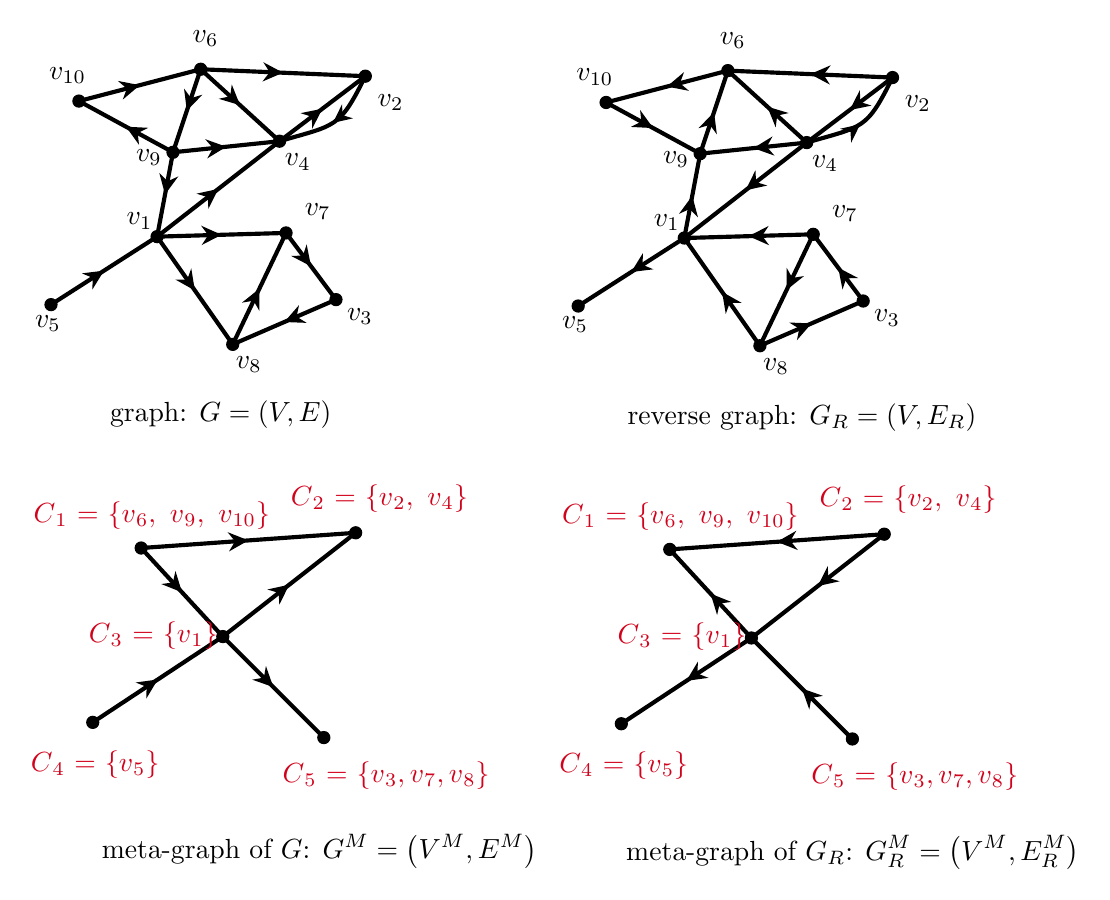
\begin{tikzpicture}[x=0.5pt,y=0.5pt,yscale=-1,xscale=1]
%uncomment if require: \path (0,615); %set diagram left start at 0, and has height of 615

%Flowchart: Connector [id:dp35531003904401826] 
\draw  [fill={rgb, 255:red, 0; green, 0; blue, 0 }  ,fill opacity=1 ] (87,378) .. controls (87,375.58) and (88.96,373.62) .. (91.38,373.62) .. controls (93.79,373.62) and (95.75,375.58) .. (95.75,378) .. controls (95.75,380.42) and (93.79,382.38) .. (91.38,382.38) .. controls (88.96,382.38) and (87,380.42) .. (87,378) -- cycle ;
%Straight Lines [id:da06413387293276729] 
\draw [color={rgb, 255:red, 0; green, 0; blue, 0 }  ,draw opacity=1 ][line width=1.5]    (114.38,92) -- (134.38,32) ;
\draw [shift={(124.38,62)}, rotate = 288.43] [fill={rgb, 255:red, 0; green, 0; blue, 0 }  ,fill opacity=1 ][line width=0.08]  [draw opacity=0] (14.56,-6.99) -- (0,0) -- (14.56,6.99) -- (9.67,0) -- cycle    ;
%Straight Lines [id:da9572573982067856] 
\draw [color={rgb, 255:red, 0; green, 0; blue, 0 }  ,draw opacity=1 ][line width=1.5]    (134.38,32) -- (46.38,55) ;
\draw [shift={(90.38,43.5)}, rotate = 165.35] [fill={rgb, 255:red, 0; green, 0; blue, 0 }  ,fill opacity=1 ][line width=0.08]  [draw opacity=0] (14.56,-6.99) -- (0,0) -- (14.56,6.99) -- (9.67,0) -- cycle    ;
%Straight Lines [id:da027017237295007268] 
\draw [color={rgb, 255:red, 0; green, 0; blue, 0 }  ,draw opacity=1 ][line width=1.5]    (150.38,442) -- (91.38,378) ;
\draw [shift={(120.88,410)}, rotate = 227.33] [fill={rgb, 255:red, 0; green, 0; blue, 0 }  ,fill opacity=1 ][line width=0.08]  [draw opacity=0] (14.56,-6.99) -- (0,0) -- (14.56,6.99) -- (9.67,0) -- cycle    ;
%Flowchart: Connector [id:dp7018202329285442] 
\draw  [fill={rgb, 255:red, 0; green, 0; blue, 0 }  ,fill opacity=1 ] (242,367) .. controls (242,364.58) and (243.96,362.62) .. (246.38,362.62) .. controls (248.79,362.62) and (250.75,364.58) .. (250.75,367) .. controls (250.75,369.42) and (248.79,371.38) .. (246.38,371.38) .. controls (243.96,371.38) and (242,369.42) .. (242,367) -- cycle ;
%Flowchart: Connector [id:dp9468304553677146] 
\draw  [fill={rgb, 255:red, 0; green, 0; blue, 0 }  ,fill opacity=1 ] (249,37) .. controls (249,34.58) and (250.96,32.62) .. (253.38,32.62) .. controls (255.79,32.62) and (257.75,34.58) .. (257.75,37) .. controls (257.75,39.42) and (255.79,41.38) .. (253.38,41.38) .. controls (250.96,41.38) and (249,39.42) .. (249,37) -- cycle ;
%Flowchart: Connector [id:dp10084257988995149] 
\draw  [fill={rgb, 255:red, 0; green, 0; blue, 0 }  ,fill opacity=1 ] (187,84) .. controls (187,81.58) and (188.96,79.62) .. (191.38,79.62) .. controls (193.79,79.62) and (195.75,81.58) .. (195.75,84) .. controls (195.75,86.42) and (193.79,88.38) .. (191.38,88.38) .. controls (188.96,88.38) and (187,86.42) .. (187,84) -- cycle ;
%Flowchart: Connector [id:dp5678652918378437] 
\draw  [fill={rgb, 255:red, 0; green, 0; blue, 0 }  ,fill opacity=1 ] (191.99,148.72) .. controls (192.85,146.46) and (195.39,145.34) .. (197.64,146.21) .. controls (199.9,147.08) and (201.02,149.61) .. (200.15,151.86) .. controls (199.28,154.12) and (196.75,155.24) .. (194.5,154.38) .. controls (192.24,153.51) and (191.12,150.97) .. (191.99,148.72) -- cycle ;
%Flowchart: Connector [id:dp9451957343710085] 
\draw  [fill={rgb, 255:red, 0; green, 0; blue, 0 }  ,fill opacity=1 ] (228.07,196.91) .. controls (228.94,194.66) and (231.47,193.53) .. (233.73,194.4) .. controls (235.98,195.27) and (237.11,197.8) .. (236.24,200.06) .. controls (235.37,202.32) and (232.84,203.44) .. (230.58,202.57) .. controls (228.33,201.7) and (227.2,199.17) .. (228.07,196.91) -- cycle ;
%Flowchart: Connector [id:dp7598246465914121] 
\draw  [fill={rgb, 255:red, 0; green, 0; blue, 0 }  ,fill opacity=1 ] (153.46,229.25) .. controls (154.33,227) and (156.86,225.87) .. (159.11,226.74) .. controls (161.37,227.61) and (162.49,230.14) .. (161.63,232.4) .. controls (160.76,234.65) and (158.22,235.78) .. (155.97,234.91) .. controls (153.71,234.04) and (152.59,231.51) .. (153.46,229.25) -- cycle ;
%Flowchart: Connector [id:dp9270593548114698] 
\draw  [fill={rgb, 255:red, 0; green, 0; blue, 0 }  ,fill opacity=1 ] (22.12,200.53) .. controls (22.99,198.28) and (25.52,197.15) .. (27.77,198.02) .. controls (30.03,198.89) and (31.15,201.42) .. (30.28,203.68) .. controls (29.42,205.94) and (26.88,207.06) .. (24.63,206.19) .. controls (22.37,205.32) and (21.25,202.79) .. (22.12,200.53) -- cycle ;
%Flowchart: Connector [id:dp0003313036349563703] 
\draw  [fill={rgb, 255:red, 0; green, 0; blue, 0 }  ,fill opacity=1 ] (98.79,151.39) .. controls (99.66,149.14) and (102.2,148.01) .. (104.45,148.88) .. controls (106.71,149.75) and (107.83,152.28) .. (106.96,154.54) .. controls (106.09,156.8) and (103.56,157.92) .. (101.3,157.05) .. controls (99.05,156.18) and (97.92,153.65) .. (98.79,151.39) -- cycle ;
%Flowchart: Connector [id:dp05524410597346219] 
\draw  [fill={rgb, 255:red, 0; green, 0; blue, 0 }  ,fill opacity=1 ] (130,32) .. controls (130,29.58) and (131.96,27.62) .. (134.38,27.62) .. controls (136.79,27.62) and (138.75,29.58) .. (138.75,32) .. controls (138.75,34.42) and (136.79,36.38) .. (134.38,36.38) .. controls (131.96,36.38) and (130,34.42) .. (130,32) -- cycle ;
%Flowchart: Connector [id:dp8722833316705884] 
\draw  [fill={rgb, 255:red, 0; green, 0; blue, 0 }  ,fill opacity=1 ] (42,55) .. controls (42,52.58) and (43.96,50.62) .. (46.38,50.62) .. controls (48.79,50.62) and (50.75,52.58) .. (50.75,55) .. controls (50.75,57.42) and (48.79,59.38) .. (46.38,59.38) .. controls (43.96,59.38) and (42,57.42) .. (42,55) -- cycle ;
%Flowchart: Connector [id:dp04902898021909796] 
\draw  [fill={rgb, 255:red, 0; green, 0; blue, 0 }  ,fill opacity=1 ] (110,92) .. controls (110,89.58) and (111.96,87.62) .. (114.38,87.62) .. controls (116.79,87.62) and (118.75,89.58) .. (118.75,92) .. controls (118.75,94.42) and (116.79,96.38) .. (114.38,96.38) .. controls (111.96,96.38) and (110,94.42) .. (110,92) -- cycle ;
%Straight Lines [id:da6957258198444844] 
\draw [color={rgb, 255:red, 0; green, 0; blue, 0 }  ,draw opacity=1 ][line width=1.5]    (46.38,55) -- (114.38,92) ;
\draw [shift={(80.38,73.5)}, rotate = 28.55] [fill={rgb, 255:red, 0; green, 0; blue, 0 }  ,fill opacity=1 ][line width=0.08]  [draw opacity=0] (14.56,-6.99) -- (0,0) -- (14.56,6.99) -- (9.67,0) -- cycle    ;
%Straight Lines [id:da1865955612168957] 
\draw [color={rgb, 255:red, 0; green, 0; blue, 0 }  ,draw opacity=1 ][line width=1.5]    (102.88,152.97) -- (114.38,92) ;
\draw [shift={(108.63,122.48)}, rotate = 280.68] [fill={rgb, 255:red, 0; green, 0; blue, 0 }  ,fill opacity=1 ][line width=0.08]  [draw opacity=0] (14.56,-6.99) -- (0,0) -- (14.56,6.99) -- (9.67,0) -- cycle    ;
%Straight Lines [id:da5983156386140572] 
\draw [color={rgb, 255:red, 0; green, 0; blue, 0 }  ,draw opacity=1 ][line width=1.5]    (102.88,152.97) -- (26.2,202.11) ;
\draw [shift={(64.54,177.54)}, rotate = 147.35] [fill={rgb, 255:red, 0; green, 0; blue, 0 }  ,fill opacity=1 ][line width=0.08]  [draw opacity=0] (14.56,-6.99) -- (0,0) -- (14.56,6.99) -- (9.67,0) -- cycle    ;
%Straight Lines [id:da7813440675788919] 
\draw [color={rgb, 255:red, 0; green, 0; blue, 0 }  ,draw opacity=1 ][line width=1.5]    (157.54,230.82) -- (102.88,152.97) ;
\draw [shift={(130.21,191.9)}, rotate = 234.93] [fill={rgb, 255:red, 0; green, 0; blue, 0 }  ,fill opacity=1 ][line width=0.08]  [draw opacity=0] (14.56,-6.99) -- (0,0) -- (14.56,6.99) -- (9.67,0) -- cycle    ;
%Straight Lines [id:da11231036470839317] 
\draw [color={rgb, 255:red, 0; green, 0; blue, 0 }  ,draw opacity=1 ][line width=1.5]    (196.07,150.29) -- (102.88,152.97) ;
\draw [shift={(149.47,151.63)}, rotate = 178.36] [fill={rgb, 255:red, 0; green, 0; blue, 0 }  ,fill opacity=1 ][line width=0.08]  [draw opacity=0] (14.56,-6.99) -- (0,0) -- (14.56,6.99) -- (9.67,0) -- cycle    ;
%Straight Lines [id:da3818914730957623] 
\draw [color={rgb, 255:red, 0; green, 0; blue, 0 }  ,draw opacity=1 ][line width=1.5]    (196.07,150.29) -- (157.54,230.82) ;
\draw [shift={(176.81,190.56)}, rotate = 115.57] [fill={rgb, 255:red, 0; green, 0; blue, 0 }  ,fill opacity=1 ][line width=0.08]  [draw opacity=0] (14.56,-6.99) -- (0,0) -- (14.56,6.99) -- (9.67,0) -- cycle    ;
%Straight Lines [id:da5617379482893489] 
\draw [color={rgb, 255:red, 0; green, 0; blue, 0 }  ,draw opacity=1 ][line width=1.5]    (157.54,230.82) -- (232.16,198.49) ;
\draw [shift={(194.85,214.66)}, rotate = 336.57] [fill={rgb, 255:red, 0; green, 0; blue, 0 }  ,fill opacity=1 ][line width=0.08]  [draw opacity=0] (14.56,-6.99) -- (0,0) -- (14.56,6.99) -- (9.67,0) -- cycle    ;
%Straight Lines [id:da7816864329937088] 
\draw [color={rgb, 255:red, 0; green, 0; blue, 0 }  ,draw opacity=1 ][line width=1.5]    (232.16,198.49) -- (196.07,150.29) ;
\draw [shift={(214.11,174.39)}, rotate = 233.18] [fill={rgb, 255:red, 0; green, 0; blue, 0 }  ,fill opacity=1 ][line width=0.08]  [draw opacity=0] (14.56,-6.99) -- (0,0) -- (14.56,6.99) -- (9.67,0) -- cycle    ;
%Straight Lines [id:da007998244336271831] 
\draw [color={rgb, 255:red, 0; green, 0; blue, 0 }  ,draw opacity=1 ][line width=1.5]    (191.38,84) -- (102.88,152.97) ;
\draw [shift={(147.13,118.48)}, rotate = 142.07] [fill={rgb, 255:red, 0; green, 0; blue, 0 }  ,fill opacity=1 ][line width=0.08]  [draw opacity=0] (14.56,-6.99) -- (0,0) -- (14.56,6.99) -- (9.67,0) -- cycle    ;
%Straight Lines [id:da07370415553910226] 
\draw [color={rgb, 255:red, 0; green, 0; blue, 0 }  ,draw opacity=1 ][line width=1.5]    (253.38,37) -- (191.38,84) ;
\draw [shift={(222.38,60.5)}, rotate = 142.84] [fill={rgb, 255:red, 0; green, 0; blue, 0 }  ,fill opacity=1 ][line width=0.08]  [draw opacity=0] (14.56,-6.99) -- (0,0) -- (14.56,6.99) -- (9.67,0) -- cycle    ;
%Straight Lines [id:da31265226854681183] 
\draw [color={rgb, 255:red, 0; green, 0; blue, 0 }  ,draw opacity=1 ][line width=1.5]    (253.38,37) -- (134.38,32) ;
\draw [shift={(193.88,34.5)}, rotate = 182.41] [fill={rgb, 255:red, 0; green, 0; blue, 0 }  ,fill opacity=1 ][line width=0.08]  [draw opacity=0] (14.56,-6.99) -- (0,0) -- (14.56,6.99) -- (9.67,0) -- cycle    ;
%Straight Lines [id:da03944598876714689] 
\draw [color={rgb, 255:red, 0; green, 0; blue, 0 }  ,draw opacity=1 ][line width=1.5]    (191.38,84) -- (114.38,92) ;
\draw [shift={(152.88,88)}, rotate = 174.07] [fill={rgb, 255:red, 0; green, 0; blue, 0 }  ,fill opacity=1 ][line width=0.08]  [draw opacity=0] (14.56,-6.99) -- (0,0) -- (14.56,6.99) -- (9.67,0) -- cycle    ;
%Curve Lines [id:da24538681443295773] 
\draw [line width=1.5]    (253.38,37) .. controls (234.5,75) and (232.5,72) .. (191.38,84) ;
\draw [shift={(229.99,70.74)}, rotate = 321.64] [fill={rgb, 255:red, 0; green, 0; blue, 0 }  ][line width=0.08]  [draw opacity=0] (13.4,-6.43) -- (0,0) -- (13.4,6.44) -- (8.9,0) -- cycle    ;
%Straight Lines [id:da5495061302418803] 
\draw [color={rgb, 255:red, 0; green, 0; blue, 0 }  ,draw opacity=1 ][line width=1.5]    (191.38,84) -- (134.38,32) ;
\draw [shift={(162.88,58)}, rotate = 222.37] [fill={rgb, 255:red, 0; green, 0; blue, 0 }  ,fill opacity=1 ][line width=0.08]  [draw opacity=0] (14.56,-6.99) -- (0,0) -- (14.56,6.99) -- (9.67,0) -- cycle    ;
%Flowchart: Connector [id:dp24932583909944328] 
\draw  [fill={rgb, 255:red, 0; green, 0; blue, 0 }  ,fill opacity=1 ] (146,442) .. controls (146,439.58) and (147.96,437.62) .. (150.38,437.62) .. controls (152.79,437.62) and (154.75,439.58) .. (154.75,442) .. controls (154.75,444.42) and (152.79,446.38) .. (150.38,446.38) .. controls (147.96,446.38) and (146,444.42) .. (146,442) -- cycle ;
%Flowchart: Connector [id:dp3666265572902413] 
\draw  [fill={rgb, 255:red, 0; green, 0; blue, 0 }  ,fill opacity=1 ] (52,504) .. controls (52,501.58) and (53.96,499.62) .. (56.38,499.62) .. controls (58.79,499.62) and (60.75,501.58) .. (60.75,504) .. controls (60.75,506.42) and (58.79,508.38) .. (56.38,508.38) .. controls (53.96,508.38) and (52,506.42) .. (52,504) -- cycle ;
%Flowchart: Connector [id:dp5809100494545972] 
\draw  [fill={rgb, 255:red, 0; green, 0; blue, 0 }  ,fill opacity=1 ] (219,515) .. controls (219,512.58) and (220.96,510.62) .. (223.38,510.62) .. controls (225.79,510.62) and (227.75,512.58) .. (227.75,515) .. controls (227.75,517.42) and (225.79,519.38) .. (223.38,519.38) .. controls (220.96,519.38) and (219,517.42) .. (219,515) -- cycle ;
%Straight Lines [id:da1229562998864333] 
\draw [color={rgb, 255:red, 0; green, 0; blue, 0 }  ,draw opacity=1 ][line width=1.5]    (246.38,367) -- (91.38,378) ;
\draw [shift={(168.88,372.5)}, rotate = 175.94] [fill={rgb, 255:red, 0; green, 0; blue, 0 }  ,fill opacity=1 ][line width=0.08]  [draw opacity=0] (14.56,-6.99) -- (0,0) -- (14.56,6.99) -- (9.67,0) -- cycle    ;
%Straight Lines [id:da6177657045500177] 
\draw [color={rgb, 255:red, 0; green, 0; blue, 0 }  ,draw opacity=1 ][line width=1.5]    (246.38,367) -- (150.38,442) ;
\draw [shift={(198.38,404.5)}, rotate = 142] [fill={rgb, 255:red, 0; green, 0; blue, 0 }  ,fill opacity=1 ][line width=0.08]  [draw opacity=0] (14.56,-6.99) -- (0,0) -- (14.56,6.99) -- (9.67,0) -- cycle    ;
%Straight Lines [id:da45439161896636415] 
\draw [color={rgb, 255:red, 0; green, 0; blue, 0 }  ,draw opacity=1 ][line width=1.5]    (223.38,515) -- (150.38,442) ;
\draw [shift={(186.88,478.5)}, rotate = 225] [fill={rgb, 255:red, 0; green, 0; blue, 0 }  ,fill opacity=1 ][line width=0.08]  [draw opacity=0] (14.56,-6.99) -- (0,0) -- (14.56,6.99) -- (9.67,0) -- cycle    ;
%Straight Lines [id:da11561285868658588] 
\draw [color={rgb, 255:red, 0; green, 0; blue, 0 }  ,draw opacity=1 ][line width=1.5]    (150.38,442) -- (56.38,504) ;
\draw [shift={(103.38,473)}, rotate = 146.59] [fill={rgb, 255:red, 0; green, 0; blue, 0 }  ,fill opacity=1 ][line width=0.08]  [draw opacity=0] (14.56,-6.99) -- (0,0) -- (14.56,6.99) -- (9.67,0) -- cycle    ;
%Straight Lines [id:da8168779159006088] 
\draw [color={rgb, 255:red, 0; green, 0; blue, 0 }  ,draw opacity=1 ][line width=1.5]    (495.38,93) -- (515.38,33) ;
\draw [shift={(505.38,63)}, rotate = 468.43] [fill={rgb, 255:red, 0; green, 0; blue, 0 }  ,fill opacity=1 ][line width=0.08]  [draw opacity=0] (14.56,-6.99) -- (0,0) -- (14.56,6.99) -- (9.67,0) -- cycle    ;
%Straight Lines [id:da894325464874] 
\draw [color={rgb, 255:red, 0; green, 0; blue, 0 }  ,draw opacity=1 ][line width=1.5]    (515.38,33) -- (427.38,56) ;
\draw [shift={(471.38,44.5)}, rotate = 345.35] [fill={rgb, 255:red, 0; green, 0; blue, 0 }  ,fill opacity=1 ][line width=0.08]  [draw opacity=0] (14.56,-6.99) -- (0,0) -- (14.56,6.99) -- (9.67,0) -- cycle    ;
%Flowchart: Connector [id:dp2028061961127232] 
\draw  [fill={rgb, 255:red, 0; green, 0; blue, 0 }  ,fill opacity=1 ] (630,38) .. controls (630,35.58) and (631.96,33.62) .. (634.38,33.62) .. controls (636.79,33.62) and (638.75,35.58) .. (638.75,38) .. controls (638.75,40.42) and (636.79,42.38) .. (634.38,42.38) .. controls (631.96,42.38) and (630,40.42) .. (630,38) -- cycle ;
%Flowchart: Connector [id:dp6685886791876837] 
\draw  [fill={rgb, 255:red, 0; green, 0; blue, 0 }  ,fill opacity=1 ] (568,85) .. controls (568,82.58) and (569.96,80.62) .. (572.38,80.62) .. controls (574.79,80.62) and (576.75,82.58) .. (576.75,85) .. controls (576.75,87.42) and (574.79,89.38) .. (572.38,89.38) .. controls (569.96,89.38) and (568,87.42) .. (568,85) -- cycle ;
%Flowchart: Connector [id:dp6828969280331417] 
\draw  [fill={rgb, 255:red, 0; green, 0; blue, 0 }  ,fill opacity=1 ] (572.99,149.72) .. controls (573.85,147.46) and (576.39,146.34) .. (578.64,147.21) .. controls (580.9,148.08) and (582.02,150.61) .. (581.15,152.86) .. controls (580.28,155.12) and (577.75,156.24) .. (575.5,155.38) .. controls (573.24,154.51) and (572.12,151.97) .. (572.99,149.72) -- cycle ;
%Flowchart: Connector [id:dp5869007902050025] 
\draw  [fill={rgb, 255:red, 0; green, 0; blue, 0 }  ,fill opacity=1 ] (609.07,197.91) .. controls (609.94,195.66) and (612.47,194.53) .. (614.73,195.4) .. controls (616.98,196.27) and (618.11,198.8) .. (617.24,201.06) .. controls (616.37,203.32) and (613.84,204.44) .. (611.58,203.57) .. controls (609.33,202.7) and (608.2,200.17) .. (609.07,197.91) -- cycle ;
%Flowchart: Connector [id:dp29745484225367824] 
\draw  [fill={rgb, 255:red, 0; green, 0; blue, 0 }  ,fill opacity=1 ] (534.46,230.25) .. controls (535.33,228) and (537.86,226.87) .. (540.11,227.74) .. controls (542.37,228.61) and (543.49,231.14) .. (542.63,233.4) .. controls (541.76,235.65) and (539.22,236.78) .. (536.97,235.91) .. controls (534.71,235.04) and (533.59,232.51) .. (534.46,230.25) -- cycle ;
%Flowchart: Connector [id:dp9007070710643801] 
\draw  [fill={rgb, 255:red, 0; green, 0; blue, 0 }  ,fill opacity=1 ] (403.12,201.53) .. controls (403.99,199.28) and (406.52,198.15) .. (408.77,199.02) .. controls (411.03,199.89) and (412.15,202.42) .. (411.28,204.68) .. controls (410.42,206.94) and (407.88,208.06) .. (405.63,207.19) .. controls (403.37,206.32) and (402.25,203.79) .. (403.12,201.53) -- cycle ;
%Flowchart: Connector [id:dp8032522319169138] 
\draw  [fill={rgb, 255:red, 0; green, 0; blue, 0 }  ,fill opacity=1 ] (479.79,152.39) .. controls (480.66,150.14) and (483.2,149.01) .. (485.45,149.88) .. controls (487.71,150.75) and (488.83,153.28) .. (487.96,155.54) .. controls (487.09,157.8) and (484.56,158.92) .. (482.3,158.05) .. controls (480.05,157.18) and (478.92,154.65) .. (479.79,152.39) -- cycle ;
%Flowchart: Connector [id:dp3269943450949304] 
\draw  [fill={rgb, 255:red, 0; green, 0; blue, 0 }  ,fill opacity=1 ] (511,33) .. controls (511,30.58) and (512.96,28.62) .. (515.38,28.62) .. controls (517.79,28.62) and (519.75,30.58) .. (519.75,33) .. controls (519.75,35.42) and (517.79,37.38) .. (515.38,37.38) .. controls (512.96,37.38) and (511,35.42) .. (511,33) -- cycle ;
%Flowchart: Connector [id:dp23422253916024505] 
\draw  [fill={rgb, 255:red, 0; green, 0; blue, 0 }  ,fill opacity=1 ] (423,56) .. controls (423,53.58) and (424.96,51.62) .. (427.38,51.62) .. controls (429.79,51.62) and (431.75,53.58) .. (431.75,56) .. controls (431.75,58.42) and (429.79,60.38) .. (427.38,60.38) .. controls (424.96,60.38) and (423,58.42) .. (423,56) -- cycle ;
%Flowchart: Connector [id:dp010586655389437372] 
\draw  [fill={rgb, 255:red, 0; green, 0; blue, 0 }  ,fill opacity=1 ] (491,93) .. controls (491,90.58) and (492.96,88.62) .. (495.38,88.62) .. controls (497.79,88.62) and (499.75,90.58) .. (499.75,93) .. controls (499.75,95.42) and (497.79,97.38) .. (495.38,97.38) .. controls (492.96,97.38) and (491,95.42) .. (491,93) -- cycle ;
%Straight Lines [id:da51057635409129] 
\draw [color={rgb, 255:red, 0; green, 0; blue, 0 }  ,draw opacity=1 ][line width=1.5]    (427.38,56) -- (495.38,93) ;
\draw [shift={(461.38,74.5)}, rotate = 208.55] [fill={rgb, 255:red, 0; green, 0; blue, 0 }  ,fill opacity=1 ][line width=0.08]  [draw opacity=0] (14.56,-6.99) -- (0,0) -- (14.56,6.99) -- (9.67,0) -- cycle    ;
%Straight Lines [id:da9705884712552635] 
\draw [color={rgb, 255:red, 0; green, 0; blue, 0 }  ,draw opacity=1 ][line width=1.5]    (483.88,153.97) -- (495.38,93) ;
\draw [shift={(489.63,123.48)}, rotate = 460.68] [fill={rgb, 255:red, 0; green, 0; blue, 0 }  ,fill opacity=1 ][line width=0.08]  [draw opacity=0] (14.56,-6.99) -- (0,0) -- (14.56,6.99) -- (9.67,0) -- cycle    ;
%Straight Lines [id:da5127893862513866] 
\draw [color={rgb, 255:red, 0; green, 0; blue, 0 }  ,draw opacity=1 ][line width=1.5]    (483.88,153.97) -- (407.2,203.11) ;
\draw [shift={(445.54,178.54)}, rotate = 327.35] [fill={rgb, 255:red, 0; green, 0; blue, 0 }  ,fill opacity=1 ][line width=0.08]  [draw opacity=0] (14.56,-6.99) -- (0,0) -- (14.56,6.99) -- (9.67,0) -- cycle    ;
%Straight Lines [id:da5716196586001995] 
\draw [color={rgb, 255:red, 0; green, 0; blue, 0 }  ,draw opacity=1 ][line width=1.5]    (538.54,231.82) -- (483.88,153.97) ;
\draw [shift={(511.21,192.9)}, rotate = 414.93] [fill={rgb, 255:red, 0; green, 0; blue, 0 }  ,fill opacity=1 ][line width=0.08]  [draw opacity=0] (14.56,-6.99) -- (0,0) -- (14.56,6.99) -- (9.67,0) -- cycle    ;
%Straight Lines [id:da9185935928544606] 
\draw [color={rgb, 255:red, 0; green, 0; blue, 0 }  ,draw opacity=1 ][line width=1.5]    (577.07,151.29) -- (483.88,153.97) ;
\draw [shift={(530.47,152.63)}, rotate = 358.36] [fill={rgb, 255:red, 0; green, 0; blue, 0 }  ,fill opacity=1 ][line width=0.08]  [draw opacity=0] (14.56,-6.99) -- (0,0) -- (14.56,6.99) -- (9.67,0) -- cycle    ;
%Straight Lines [id:da5526780501990177] 
\draw [color={rgb, 255:red, 0; green, 0; blue, 0 }  ,draw opacity=1 ][line width=1.5]    (577.07,151.29) -- (538.54,231.82) ;
\draw [shift={(557.81,191.56)}, rotate = 295.57] [fill={rgb, 255:red, 0; green, 0; blue, 0 }  ,fill opacity=1 ][line width=0.08]  [draw opacity=0] (14.56,-6.99) -- (0,0) -- (14.56,6.99) -- (9.67,0) -- cycle    ;
%Straight Lines [id:da07669648878710078] 
\draw [color={rgb, 255:red, 0; green, 0; blue, 0 }  ,draw opacity=1 ][line width=1.5]    (538.54,231.82) -- (613.16,199.49) ;
\draw [shift={(575.85,215.66)}, rotate = 516.5699999999999] [fill={rgb, 255:red, 0; green, 0; blue, 0 }  ,fill opacity=1 ][line width=0.08]  [draw opacity=0] (14.56,-6.99) -- (0,0) -- (14.56,6.99) -- (9.67,0) -- cycle    ;
%Straight Lines [id:da04407384927929969] 
\draw [color={rgb, 255:red, 0; green, 0; blue, 0 }  ,draw opacity=1 ][line width=1.5]    (613.16,199.49) -- (577.07,151.29) ;
\draw [shift={(595.11,175.39)}, rotate = 413.18] [fill={rgb, 255:red, 0; green, 0; blue, 0 }  ,fill opacity=1 ][line width=0.08]  [draw opacity=0] (14.56,-6.99) -- (0,0) -- (14.56,6.99) -- (9.67,0) -- cycle    ;
%Straight Lines [id:da7736173583087967] 
\draw [color={rgb, 255:red, 0; green, 0; blue, 0 }  ,draw opacity=1 ][line width=1.5]    (572.38,85) -- (483.88,153.97) ;
\draw [shift={(528.13,119.48)}, rotate = 322.07] [fill={rgb, 255:red, 0; green, 0; blue, 0 }  ,fill opacity=1 ][line width=0.08]  [draw opacity=0] (14.56,-6.99) -- (0,0) -- (14.56,6.99) -- (9.67,0) -- cycle    ;
%Straight Lines [id:da984046162104014] 
\draw [color={rgb, 255:red, 0; green, 0; blue, 0 }  ,draw opacity=1 ][line width=1.5]    (634.38,38) -- (572.38,85) ;
\draw [shift={(603.38,61.5)}, rotate = 322.84000000000003] [fill={rgb, 255:red, 0; green, 0; blue, 0 }  ,fill opacity=1 ][line width=0.08]  [draw opacity=0] (14.56,-6.99) -- (0,0) -- (14.56,6.99) -- (9.67,0) -- cycle    ;
%Straight Lines [id:da41303131230822765] 
\draw [color={rgb, 255:red, 0; green, 0; blue, 0 }  ,draw opacity=1 ][line width=1.5]    (634.38,38) -- (515.38,33) ;
\draw [shift={(574.88,35.5)}, rotate = 362.40999999999997] [fill={rgb, 255:red, 0; green, 0; blue, 0 }  ,fill opacity=1 ][line width=0.08]  [draw opacity=0] (14.56,-6.99) -- (0,0) -- (14.56,6.99) -- (9.67,0) -- cycle    ;
%Straight Lines [id:da9312483814272712] 
\draw [color={rgb, 255:red, 0; green, 0; blue, 0 }  ,draw opacity=1 ][line width=1.5]    (572.38,85) -- (495.38,93) ;
\draw [shift={(533.88,89)}, rotate = 354.07] [fill={rgb, 255:red, 0; green, 0; blue, 0 }  ,fill opacity=1 ][line width=0.08]  [draw opacity=0] (14.56,-6.99) -- (0,0) -- (14.56,6.99) -- (9.67,0) -- cycle    ;
%Curve Lines [id:da6657670157747444] 
\draw [line width=1.5]    (634.38,38) .. controls (615.5,76) and (613.5,73) .. (572.38,85) ;
\draw [shift={(610.99,71.74)}, rotate = 141.64] [fill={rgb, 255:red, 0; green, 0; blue, 0 }  ][line width=0.08]  [draw opacity=0] (13.4,-6.43) -- (0,0) -- (13.4,6.44) -- (8.9,0) -- cycle    ;
%Straight Lines [id:da6019953764665212] 
\draw [color={rgb, 255:red, 0; green, 0; blue, 0 }  ,draw opacity=1 ][line width=1.5]    (572.38,85) -- (515.38,33) ;
\draw [shift={(543.88,59)}, rotate = 402.37] [fill={rgb, 255:red, 0; green, 0; blue, 0 }  ,fill opacity=1 ][line width=0.08]  [draw opacity=0] (14.56,-6.99) -- (0,0) -- (14.56,6.99) -- (9.67,0) -- cycle    ;
%Flowchart: Connector [id:dp2447453141676298] 
\draw  [fill={rgb, 255:red, 0; green, 0; blue, 0 }  ,fill opacity=1 ] (469,379) .. controls (469,376.58) and (470.96,374.62) .. (473.38,374.62) .. controls (475.79,374.62) and (477.75,376.58) .. (477.75,379) .. controls (477.75,381.42) and (475.79,383.38) .. (473.38,383.38) .. controls (470.96,383.38) and (469,381.42) .. (469,379) -- cycle ;
%Straight Lines [id:da8606033691768754] 
\draw [color={rgb, 255:red, 0; green, 0; blue, 0 }  ,draw opacity=1 ][line width=1.5]    (532.38,443) -- (473.38,379) ;
\draw [shift={(502.88,411)}, rotate = 407.33000000000004] [fill={rgb, 255:red, 0; green, 0; blue, 0 }  ,fill opacity=1 ][line width=0.08]  [draw opacity=0] (14.56,-6.99) -- (0,0) -- (14.56,6.99) -- (9.67,0) -- cycle    ;
%Flowchart: Connector [id:dp591146190566066] 
\draw  [fill={rgb, 255:red, 0; green, 0; blue, 0 }  ,fill opacity=1 ] (624,368) .. controls (624,365.58) and (625.96,363.62) .. (628.38,363.62) .. controls (630.79,363.62) and (632.75,365.58) .. (632.75,368) .. controls (632.75,370.42) and (630.79,372.38) .. (628.38,372.38) .. controls (625.96,372.38) and (624,370.42) .. (624,368) -- cycle ;
%Flowchart: Connector [id:dp231499536937802] 
\draw  [fill={rgb, 255:red, 0; green, 0; blue, 0 }  ,fill opacity=1 ] (528,443) .. controls (528,440.58) and (529.96,438.62) .. (532.38,438.62) .. controls (534.79,438.62) and (536.75,440.58) .. (536.75,443) .. controls (536.75,445.42) and (534.79,447.38) .. (532.38,447.38) .. controls (529.96,447.38) and (528,445.42) .. (528,443) -- cycle ;
%Flowchart: Connector [id:dp47523679634028715] 
\draw  [fill={rgb, 255:red, 0; green, 0; blue, 0 }  ,fill opacity=1 ] (434,505) .. controls (434,502.58) and (435.96,500.62) .. (438.38,500.62) .. controls (440.79,500.62) and (442.75,502.58) .. (442.75,505) .. controls (442.75,507.42) and (440.79,509.38) .. (438.38,509.38) .. controls (435.96,509.38) and (434,507.42) .. (434,505) -- cycle ;
%Flowchart: Connector [id:dp593330998531193] 
\draw  [fill={rgb, 255:red, 0; green, 0; blue, 0 }  ,fill opacity=1 ] (601,516) .. controls (601,513.58) and (602.96,511.62) .. (605.38,511.62) .. controls (607.79,511.62) and (609.75,513.58) .. (609.75,516) .. controls (609.75,518.42) and (607.79,520.38) .. (605.38,520.38) .. controls (602.96,520.38) and (601,518.42) .. (601,516) -- cycle ;
%Straight Lines [id:da05923813499561881] 
\draw [color={rgb, 255:red, 0; green, 0; blue, 0 }  ,draw opacity=1 ][line width=1.5]    (628.38,368) -- (473.38,379) ;
\draw [shift={(550.88,373.5)}, rotate = 355.94] [fill={rgb, 255:red, 0; green, 0; blue, 0 }  ,fill opacity=1 ][line width=0.08]  [draw opacity=0] (14.56,-6.99) -- (0,0) -- (14.56,6.99) -- (9.67,0) -- cycle    ;
%Straight Lines [id:da4311696280051074] 
\draw [color={rgb, 255:red, 0; green, 0; blue, 0 }  ,draw opacity=1 ][line width=1.5]    (628.38,368) -- (532.38,443) ;
\draw [shift={(580.38,405.5)}, rotate = 322] [fill={rgb, 255:red, 0; green, 0; blue, 0 }  ,fill opacity=1 ][line width=0.08]  [draw opacity=0] (14.56,-6.99) -- (0,0) -- (14.56,6.99) -- (9.67,0) -- cycle    ;
%Straight Lines [id:da8663749303427544] 
\draw [color={rgb, 255:red, 0; green, 0; blue, 0 }  ,draw opacity=1 ][line width=1.5]    (605.38,516) -- (532.38,443) ;
\draw [shift={(568.88,479.5)}, rotate = 405] [fill={rgb, 255:red, 0; green, 0; blue, 0 }  ,fill opacity=1 ][line width=0.08]  [draw opacity=0] (14.56,-6.99) -- (0,0) -- (14.56,6.99) -- (9.67,0) -- cycle    ;
%Straight Lines [id:da34096248111738436] 
\draw [color={rgb, 255:red, 0; green, 0; blue, 0 }  ,draw opacity=1 ][line width=1.5]    (532.38,443) -- (438.38,505) ;
\draw [shift={(485.38,474)}, rotate = 326.59000000000003] [fill={rgb, 255:red, 0; green, 0; blue, 0 }  ,fill opacity=1 ][line width=0.08]  [draw opacity=0] (14.56,-6.99) -- (0,0) -- (14.56,6.99) -- (9.67,0) -- cycle    ;

% Text Node
\draw (79,134) node [anchor=north west][inner sep=0.75pt]   [align=left] {$\displaystyle v_{1}$};
% Text Node
\draw (238.24,203.06) node [anchor=north west][inner sep=0.75pt]   [align=left] {$\displaystyle v_{3}$};
% Text Node
\draw (12.75,208) node [anchor=north west][inner sep=0.75pt]   [align=left] {$\displaystyle v_{5}$};
% Text Node
\draw (193.38,91.38) node [anchor=north west][inner sep=0.75pt]   [align=left] {$\displaystyle v_{4}$};
% Text Node
\draw (260.38,48.38) node [anchor=north west][inner sep=0.75pt]   [align=left] {$\displaystyle v_{2}$};
% Text Node
\draw (126.75,2.35) node [anchor=north west][inner sep=0.75pt]   [align=left] {$\displaystyle v_{6}$};
% Text Node
\draw (207.75,127.35) node [anchor=north west][inner sep=0.75pt]   [align=left] {$\displaystyle v_{7}$};
% Text Node
\draw (67,269.93) node [anchor=north west][inner sep=0.75pt]   [align=left] {graph: $\displaystyle G=( V,E)$};
% Text Node
\draw (157.97,237.91) node [anchor=north west][inner sep=0.75pt]   [align=left] {$\displaystyle v_{8}$};
% Text Node
\draw (22.97,28.91) node [anchor=north west][inner sep=0.75pt]   [align=left] {$\displaystyle v_{10}$};
% Text Node
\draw (85.75,88.35) node [anchor=north west][inner sep=0.75pt]   [align=left] {$\displaystyle v_{9}$};
% Text Node
\draw (11.75,342.35) node [anchor=north west][inner sep=0.75pt]   [align=left] {$\displaystyle \textcolor[rgb]{0.82,0.01,0.11}{C}\textcolor[rgb]{0.82,0.01,0.11}{_{1}}\textcolor[rgb]{0.82,0.01,0.11}{\ =\ }\textcolor[rgb]{0.82,0.01,0.11}{\{}\textcolor[rgb]{0.82,0.01,0.11}{v}\textcolor[rgb]{0.82,0.01,0.11}{_{6}}\textcolor[rgb]{0.82,0.01,0.11}{,\ v}\textcolor[rgb]{0.82,0.01,0.11}{_{9}}\textcolor[rgb]{0.82,0.01,0.11}{,\ v}\textcolor[rgb]{0.82,0.01,0.11}{_{10}}\textcolor[rgb]{0.82,0.01,0.11}{\}}$};
% Text Node
\draw (197.75,330.35) node [anchor=north west][inner sep=0.75pt]   [align=left] {$\displaystyle \textcolor[rgb]{0.82,0.01,0.11}{C}\textcolor[rgb]{0.82,0.01,0.11}{_{2}}\textcolor[rgb]{0.82,0.01,0.11}{\ =\ }\textcolor[rgb]{0.82,0.01,0.11}{\{}\textcolor[rgb]{0.82,0.01,0.11}{v}\textcolor[rgb]{0.82,0.01,0.11}{_{2}}\textcolor[rgb]{0.82,0.01,0.11}{,\ v}\textcolor[rgb]{0.82,0.01,0.11}{_{4}}\textcolor[rgb]{0.82,0.01,0.11}{\}}$};
% Text Node
\draw (51.75,429.35) node [anchor=north west][inner sep=0.75pt]   [align=left] {$\displaystyle \textcolor[rgb]{0.82,0.01,0.11}{C}\textcolor[rgb]{0.82,0.01,0.11}{_{3}}\textcolor[rgb]{0.82,0.01,0.11}{\ =\ }\textcolor[rgb]{0.82,0.01,0.11}{\{}\textcolor[rgb]{0.82,0.01,0.11}{v}\textcolor[rgb]{0.82,0.01,0.11}{_{1}}\textcolor[rgb]{0.82,0.01,0.11}{\}}$};
% Text Node
\draw (9.75,522.35) node [anchor=north west][inner sep=0.75pt]   [align=left] {$\displaystyle \textcolor[rgb]{0.82,0.01,0.11}{C}\textcolor[rgb]{0.82,0.01,0.11}{_{4}}\textcolor[rgb]{0.82,0.01,0.11}{\ =\ }\textcolor[rgb]{0.82,0.01,0.11}{\{}\textcolor[rgb]{0.82,0.01,0.11}{v}\textcolor[rgb]{0.82,0.01,0.11}{_{5}}\textcolor[rgb]{0.82,0.01,0.11}{\}}$};
% Text Node
\draw (191.75,530.35) node [anchor=north west][inner sep=0.75pt]   [align=left] {$\displaystyle \textcolor[rgb]{0.82,0.01,0.11}{C}\textcolor[rgb]{0.82,0.01,0.11}{_{5}}\textcolor[rgb]{0.82,0.01,0.11}{\ =\ }\textcolor[rgb]{0.82,0.01,0.11}{\{}\textcolor[rgb]{0.82,0.01,0.11}{v}\textcolor[rgb]{0.82,0.01,0.11}{_{3}}\textcolor[rgb]{0.82,0.01,0.11}{,v}\textcolor[rgb]{0.82,0.01,0.11}{_{7}}\textcolor[rgb]{0.82,0.01,0.11}{,v}\textcolor[rgb]{0.82,0.01,0.11}{_{8}}\textcolor[rgb]{0.82,0.01,0.11}{\}}$};
% Text Node
\draw (61,582.93) node [anchor=north west][inner sep=0.75pt]   [align=left] {meta-graph of $\displaystyle G$: $\displaystyle G^{M} =\left( V^{M} ,E^{M}\right)$};
% Text Node
\draw (460,135) node [anchor=north west][inner sep=0.75pt]   [align=left] {$\displaystyle v_{1}$};
% Text Node
\draw (619.24,204.06) node [anchor=north west][inner sep=0.75pt]   [align=left] {$\displaystyle v_{3}$};
% Text Node
\draw (393.75,209) node [anchor=north west][inner sep=0.75pt]   [align=left] {$\displaystyle v_{5}$};
% Text Node
\draw (574.38,92.38) node [anchor=north west][inner sep=0.75pt]   [align=left] {$\displaystyle v_{4}$};
% Text Node
\draw (641.38,49.38) node [anchor=north west][inner sep=0.75pt]   [align=left] {$\displaystyle v_{2}$};
% Text Node
\draw (507.75,3.35) node [anchor=north west][inner sep=0.75pt]   [align=left] {$\displaystyle v_{6}$};
% Text Node
\draw (588.75,128.35) node [anchor=north west][inner sep=0.75pt]   [align=left] {$\displaystyle v_{7}$};
% Text Node
\draw (441,271.93) node [anchor=north west][inner sep=0.75pt]   [align=left] {reverse graph: $\displaystyle G_{R} =( V,E_{R})$};
% Text Node
\draw (538.97,238.91) node [anchor=north west][inner sep=0.75pt]   [align=left] {$\displaystyle v_{8}$};
% Text Node
\draw (403.97,29.91) node [anchor=north west][inner sep=0.75pt]   [align=left] {$\displaystyle v_{10}$};
% Text Node
\draw (466.75,89.35) node [anchor=north west][inner sep=0.75pt]   [align=left] {$\displaystyle v_{9}$};
% Text Node
\draw (393.75,343.35) node [anchor=north west][inner sep=0.75pt]   [align=left] {$\displaystyle \textcolor[rgb]{0.82,0.01,0.11}{C}\textcolor[rgb]{0.82,0.01,0.11}{_{1}}\textcolor[rgb]{0.82,0.01,0.11}{\ =\ }\textcolor[rgb]{0.82,0.01,0.11}{\{}\textcolor[rgb]{0.82,0.01,0.11}{v}\textcolor[rgb]{0.82,0.01,0.11}{_{6}}\textcolor[rgb]{0.82,0.01,0.11}{,\ v}\textcolor[rgb]{0.82,0.01,0.11}{_{9}}\textcolor[rgb]{0.82,0.01,0.11}{,\ v}\textcolor[rgb]{0.82,0.01,0.11}{_{10}}\textcolor[rgb]{0.82,0.01,0.11}{\}}$};
% Text Node
\draw (579.75,331.35) node [anchor=north west][inner sep=0.75pt]   [align=left] {$\displaystyle \textcolor[rgb]{0.82,0.01,0.11}{C}\textcolor[rgb]{0.82,0.01,0.11}{_{2}}\textcolor[rgb]{0.82,0.01,0.11}{\ =\ }\textcolor[rgb]{0.82,0.01,0.11}{\{}\textcolor[rgb]{0.82,0.01,0.11}{v}\textcolor[rgb]{0.82,0.01,0.11}{_{2}}\textcolor[rgb]{0.82,0.01,0.11}{,\ v}\textcolor[rgb]{0.82,0.01,0.11}{_{4}}\textcolor[rgb]{0.82,0.01,0.11}{\}}$};
% Text Node
\draw (433.75,430.35) node [anchor=north west][inner sep=0.75pt]   [align=left] {$\displaystyle \textcolor[rgb]{0.82,0.01,0.11}{C}\textcolor[rgb]{0.82,0.01,0.11}{_{3}}\textcolor[rgb]{0.82,0.01,0.11}{\ =\ }\textcolor[rgb]{0.82,0.01,0.11}{\{}\textcolor[rgb]{0.82,0.01,0.11}{v}\textcolor[rgb]{0.82,0.01,0.11}{_{1}}\textcolor[rgb]{0.82,0.01,0.11}{\}}$};
% Text Node
\draw (391.75,523.35) node [anchor=north west][inner sep=0.75pt]   [align=left] {$\displaystyle \textcolor[rgb]{0.82,0.01,0.11}{C}\textcolor[rgb]{0.82,0.01,0.11}{_{4}}\textcolor[rgb]{0.82,0.01,0.11}{\ =\ }\textcolor[rgb]{0.82,0.01,0.11}{\{}\textcolor[rgb]{0.82,0.01,0.11}{v}\textcolor[rgb]{0.82,0.01,0.11}{_{5}}\textcolor[rgb]{0.82,0.01,0.11}{\}}$};
% Text Node
\draw (573.75,531.35) node [anchor=north west][inner sep=0.75pt]   [align=left] {$\displaystyle \textcolor[rgb]{0.82,0.01,0.11}{C}\textcolor[rgb]{0.82,0.01,0.11}{_{5}}\textcolor[rgb]{0.82,0.01,0.11}{\ =\ }\textcolor[rgb]{0.82,0.01,0.11}{\{}\textcolor[rgb]{0.82,0.01,0.11}{v}\textcolor[rgb]{0.82,0.01,0.11}{_{3}}\textcolor[rgb]{0.82,0.01,0.11}{,v}\textcolor[rgb]{0.82,0.01,0.11}{_{7}}\textcolor[rgb]{0.82,0.01,0.11}{,v}\textcolor[rgb]{0.82,0.01,0.11}{_{8}}\textcolor[rgb]{0.82,0.01,0.11}{\}}$};
% Text Node
\draw (440,583.93) node [anchor=north west][inner sep=0.75pt]   [align=left] {meta-graph of $\displaystyle G_{R}$: $\displaystyle G^{M}_{R} =\left( V^{M} ,E^{M}_{R}\right)$};


\end{tikzpicture}

}
\caption{Graph and its reverse graph, and the corresponding meta-graphs.}
\label{fig:reverse}
\end{figure}

Following properties can be easily proved using above definition.

\begin{property}
There is a path from $u$ to $v$ in $G$ if and only if there is a path from $v$ to $u$ in $G_R$.
In other words, $u$ can reach $v$ in $G$ if and only if $u$ can be reached from $v$ in $G_R$.
\end{property}

\begin{property}
$(G_R)_R = G$.
\end{property}

\begin{property}
A vertex $v$ of DAG $G$ is a source vertex if and only if $v$ is a sink vertex of $G_R$.
\end{property}


\begin{property}
$G$ and $G_R$ has the same set of connected components. %In other words the meta-graph of $G$ has the same set of vertices with the meta-graph of $G_R$.
\end{property}


\begin{property}
The meta-graph of $G_R$ is the reverse graph of the meta-graph of $G$. Formally, $(G_R)^M = (G^M)_R$.
\end{property}

\begin{property}
$X$ is a linearization of DAG $G$ if and only if the reverse of $X$ is a linearization of $G_R$~(or, $X$ is a reverse-linearization of $G_R$).
In particular, since any meta-graph is a DAG, we have that 
$X$ is linearization of $G^M$ if and only if $X$ is a reverse-linearization of $(G^M)_R = (G_R)^M$,
and that $X$ is a linearization of $(G_R)^M = (G^M)_R$ if and only if $X$ is a reverse-linearization of $G^M$.
\end{property}


\section*{Algorithm to Determine Connected Components in Directed Graphs}

Combining above DFS-with-timing and reverse graph, here is the pseudo-code we use to obtain a special ordering.
The key is that we run DFS-with-timing on the reverse graph $G_R$, instead of on the given graph $G$.

\begin{minipage}{0.8\textwidth}
	\aaA {4}{Algorithm to determine the \textcolor{blue}{specific order}}\xxx
	\aab {build $G_R$ of $G$;}\xxx
	\aab {run DFS with timing on $G_R$ to get $postlist$;}\xxx
	\aab {return $postlist$;}\xxx
	\aaa {end algorithm;}\xxx
\end{minipage}

We now show that, above $postlist$, i.e., the $postlist$ obtained by running DFS-with-timing on $G_R$,
satisfies the condition that ``the ordering of connected components sorted by their first appearance in above
$postlist$ forms a reverse-linearization of the meta-graph $G_M$''.
In fact, since above $postlist$ is obtained by running DFS-with-timing on $G_R$,
according to Corollary~\ref{col2}, 
the list of all connected components sorted by their first appearance of in above $postlist$ is a linearization of $(G_R)^M$.
According to Property~6 of reverse graph, we know that a linearization of $(G_R)^M$ is a reverse-linearization of $G_M$.

Above $postlist$ can then be used by the DFS algorithm as a special order to obtain all connected components, with pseudo-code copied below.

\begin{minipage}{0.8\textwidth}
	\aaA {8}{function DFS ($G = (V, E)$)}\xxx
	\aab {num-cc = 0;}\xxx
	\aaB {5}{for \textcolor{blue}{$v_i$ in the $postlist$ obtained above}}\xxx
	\aaC {3}{if ($visited[i] = 0$)}\xxx
	\aad {num-cc = num-cc + 1;}\xxx
	\aad {explore ($G, v_j$);}\xxx
	\aac {end if;}\xxx
	\aab {end for;}\xxx
	\aaa {end algorithm;}\xxx
\end{minipage}

\begin{minipage}{0.8\textwidth}
	\aaA {5}{function explore ($G = (V, E), v_i \in V$)}\xxx
	\aab {$visited[i] = $ num-cc;}\xxx
	\aaB {2}{for any edge $(v_i, v_j) \in E$}\xxx
	\aac {if ($visited[j] = 0$): explore ($G, v_j$);}\xxx
	\aab {end for;}\xxx
	\aaa {end algorithm;}\xxx
\end{minipage}


The entire algorithm runs in $\Theta(|V| + |E|)$ time.
